%%%%%%%%%%%%%%%%%%%%%%%%%%%%% Define Article %%%%%%%%%%%%%%%%%%%%%%%%%%%%%%%%%%
\documentclass[a4paper]{article}
%%%%%%%%%%%%%%%%%%%%%%%%%%%%%%%%%%%%%%%%%%%%%%%%%%%%%%%%%%%%%%%%%%%%%%%%%%%%%%%

%%%%%%%%%%%%%%%%%%%%%%%%%%%%% Using Packages %%%%%%%%%%%%%%%%%%%%%%%%%%%%%%%%%%
\usepackage{geometry}
\usepackage{graphicx}
\usepackage{amssymb}
\usepackage{amsmath}
\usepackage{amsthm}
\usepackage{booktabs}
\usepackage{lipsum}
\usepackage{graphicx}
\usepackage{color}
\usepackage{nth}
\usepackage{bm}
\usepackage{caption}
\usepackage{subcaption}
\usepackage{url}
\usepackage{array}
\usepackage{multirow}
\usepackage{parskip}
%%%%%%%%%%%%%%%%%%%%%%%%%% Page Setting %%%%%%%%%%%%%%%%%%%%%%%%%%%%%%%%%%%%%%%
\geometry{a4paper}

% sans-serif font
\renewcommand{\familydefault}{\sfdefault}

%%%%%%%%%%%%%%%%%%%%%%%%%% Define some useful colors %%%%%%%%%%%%%%%%%%%%%%%%%%
\definecolor{ocre}{RGB}{243,102,25}
\definecolor{mygray}{RGB}{243,243,244}
\definecolor{deepGreen}{RGB}{26,111,0}
\definecolor{shallowGreen}{RGB}{235,255,255}
\definecolor{deepBlue}{RGB}{61,124,222}
\definecolor{shallowBlue}{RGB}{235,249,255}
%%%%%%%%%%%%%%%%%%%%%%%%%%%%%%%%%%%%%%%%%%%%%%%%%%%%%%%%%%%%%%%%%%%%%%%%%%%%%%%

%%%%%%%%%%%%%%%%%%%%%%%%%% Macros %%%%%%%%%%%%%%%%%%%%%%%%%%%%%%%%%%%%%%%%%%%%%
\DeclareMathOperator{\Lagr}{\mathcal{L}}
%%%%%%%%%%%%%%%%%%%%%%%%%%%%%%%%%%%%%%%%%%%%%%%%%%%%%%%%%%%%%%%%%%%%%%%%%%%%%%%


\begin{document}
  % custom title page
  \begin{titlepage}
  \begin{center}

    \vspace*{1cm}

    \textbf{\LARGE
    % Training and Deploying Computer Vision Models for Indoor Localisation
    % Exploring Deep Learning for Indoor Localisation: A Study on Room-Level Accuracy
    Navigating Indoors with Computer Vision: Exploring Deep Learning Approaches
    for Room-Level Indoor Localisation
    % Deep Learning for Accurate Room-Level Indoor Localisation: Feasibility and Evaluation
    % Enhancing Indoor Spatial Awareness: Deep Learning Approaches for Room-Level
    % Indoor Localisation
    }

    \vspace{1.5cm}

    % author
    \begin{minipage}[t]{5cm}
      \centering
      \textbf{Mika Senghaas} (Author) \\
      IT University of Copenhagen \\
      \textit{jsen@itu.dk}
    \end{minipage}
    \hspace{1cm}
    \begin{minipage}[t]{5cm}
      \centering
      \textbf{Stella Grasshof} (Supervisor) \\
      IT University of Copenhagen \\
      \textit{stgr@itu.dk}
    \end{minipage}

    \vfill

    % degree
    A Thesis presented for the Degree of \\
    \textbf{Bachelor of Science in Data Science}

    \vspace{0.8cm}

    
\includegraphics[width=0.4\textwidth]{figures/itu.jpg}

    \vspace{0.8cm}

    \textbf{IT University of Copenhagen}\\
    Computer Science Department\\
    \vspace{.5cm}
    May, 15th 2023

  \end{center}
\end{titlepage}

  \newpage

  % table of contents, list of tables, list of figures
  \tableofcontents
  % \listoftables
  % \listoffigures
  \newpage

  % Deep residual networks have emerged as a family of extremely deep
  % architectures showing compelling accuracy and nice convergence behaviors. In
  % this paper, we analyze the propagation formulations behind the residual
  % building blocks, which suggest that the forward and backward signals can be
  % directly propagated from one block to any other block, when using identity
  % mappings as the skip connections and after-addition activation. A series of
  % ablation experiments support the importance of these identity mappings. This
  % motivates us to propose a new residual unit, which makes training easier and
  % improves generalization. We report improved results using a 1001-layer ResNet
  % on CIFAR-10 (4.62% error) and CIFAR-100, and a 200-layer ResNet on ImageNet.
  % Code is available at: https://github.com/KaimingHe/resnet-1k-layers

  \begin{abstract} % (fold)

    Current indoor localisation techniques require rigorous fine-tuning to the
    task at hand, high maintenance efforts and don’t scale well, making
    commercial applications rare. In this context, and in the light of the
    success of deep learning in numerous computer vision tasks, this study
    proposes to phrase indoor localisation as a classification task in
    applications which do not require centimetre-level accuracy. Various
    traditional and state-of-the-art deep learning models, including 2D and 3D
    convolutional, residual, densely connected and self-attention based models,
    are trained and evaluated on a self-collected indoor localisation dataset.
    We show that best performing models show capabilities for generalisation and
    robustness to varying input in a low-resource data setting - giving hope
    for this approach to become a viable alternative to existing techniques.

  \end{abstract}

  \section{Introduction}
  \label{sec:introduction}

  % outdoor localisation as solved problem 
  With the introduction of GPS (Global Positioning System), a satellite-based
  positioning system, localisation in outdoor spaces has become more efficient
  and accurate than ever before. Gradual commercialisation led to the technology
  rapidly transforming industries and personal navigation. Today, outdoor
  localisation is widely considered a \textit{solved problem}.

  % gps struggles in indoor spaces
  The same cannot be said for indoor localisation. Because the transmitted radio
  signals sent out by the satellites in GPS systems are not strong enough to
  penetrate through walls and struggle with reflections from large buildings,
  the technology yields inaccurate results at best, and often becomes
  dysfunctional in indoor spaces~\textit{[CITE]}.

  % indoor localisation techniques (broad overview)
  Finding alternative solutions to provide an accurate, cheap and robust indoor
  localisation systems has been a main focus of research in the past decades,
  and is becoming increasingly important in the light of the ongoing
  urbanisation of our living spaces and the emergence of autonomous robots and
  vehicles in our everyday life. Decades of research have led to the development
  of a variety of different indoor localisation technologies. Hardware-based
  systems use radio signals, transmitted by beacons, like
  Bluetooth~\cite{bluetooth1, bluetooth2}, and Ultra-Wideband (UWB)~\cite{uwb1,
  uwb2} or Wi-Fi~\cite{survey1, survey2, wireless-positioning}, to localise an
  agent in a known environment. Software-based systems, like Simultaneous
  Localisation and Mapping (SLAM)~\cite{mono-slam, ptam, orb-slam} algorithms,
  use sensory information, like cameras or distance-measuring laser sensors, as
  input to a complex pipeline involving various computer vision algorithms to
  ultimately localise an agent in an unknown environment, while also building a
  map of the environment.
  
  % short-comings of existing approaches
  While these approaches have proven to produce remarkable results, being
  capable of localising an agent with centimetre accuracy, they are limited for
  various reasons: Hardware-based system require an expensive initial setup,
  continuous maintenance of the signal-transmitting beacons, and are often not
  feasible in large environments~\textit{[CITE]}. SLAM algorithms, on the other
  hand, require a meticulously handcrafted pipeline of feature detection,
  feature matching, and pose estimation that has to be fine-tuned by experts for
  each indoor space, to achieve outstanding results~\textit{[CITE]}. All of the
  above short-comings of existing indoor localisation technologies make
  commercial applications rare and not unified in their approach. 

  % short-comings of existing approaches
  All of the above approaches work under the assumption that centimetre-accuracy
  is required for indoor localisation. However, this is not always the case. For
  some applications, like indoor navigation, it is sufficient to know the
  position of the agent with a meter or even room-accuracy, instead of
  centimetre accuracy. One example of such an application is the navigation in
  large indoor spaces, like airports, train stations, or shopping malls, where
  the goal is to guide the agent to a specific room or area. In these cases, the
  constraint of centimetre-accuracy can be relaxed, in favour of a simpler and
  more versatile solution.

  % success of deep learning in computer vision
  In the past decades, deep learning has proven to be a powerful tool in a
  wide-variety of tasks and has repeatedly proven remarkable capabilities in the
  field of computer vision. Amongst common tasks in computer vision are the tasks
  of image and video classification, where the goal is to predict a label from a
  set of pre-defined labels for a given image or video.

  % deep learning for indoor localisation
  Motivated by the apparent lack of a simple, unified indoor localisation system
  and the success of deep learning in computer vision, this study investigates
  the applicability of modern deep learning techniques to the task of indoor
  localisation when viewing localisation as a classification task. The study
  presents the rigorous evaluation of several modern deep learning architectures
  on a challengingly small video dataset for mapping out a novel indoor space.

  % section introduction (end)

  \section{Background} % (fold)
  \label{sec:background}

  Creating accurate, robust and cheap indoor localisation systems is not a novel
  task, but has been a focus of research at the intersection of robotics,
  computer vision and machine learning for decades.

  \subsection{Hardware-Based Indoor Localisation} % (fold)
  \label{sub:hardware-based-indoor-localisation}

  The approach conceptually closest to GPS-based outdoor localisation systems
  are hardware-based indoor localisation systems. Because radio signals
  transmitted by satellites are incapable of penetrating through walls, various
  close-proximity radio signals have been proposed to be used for indoor
  localisation, such as Bluetooth~\cite{bluetooth1, bluetooth2}, Ultra-Wideband
  (UWB)~\cite{uwb1, uwb2} or Wi-Fi~\cite{survey1, survey2}.

  No matter the radio signals, three main approaches can be distinguished:
  (1) Angle of Arrival (AOA), (2) Time of Arrival (TOA) and (3)
  RSSI-Fingerprinting (RSSI-FP)~\cite{survey2}. 

  In AOA approaches, transmitting beacons, called access points (APs), are
  measuring the distance and angle between a beacon and an agent. The
  intersection between the lines of sight (LoS) of at least three APs yields
  the position of the agent. 

  TOA approaches (such as GPS) use the received signal strength (RSS) to
  estimate the distance between an agent and the AP through a propagation model.
  Given the distance estimates of at least four APs, the agent's position can be
  determined by an approach called multilateration, which is based on the idea
  that an agent's position in three-dimensional space can be uniquely determined
  by the intersection of four spheres with known radius and centres. Clearly,
  TOA approaches require knowledge about the position of the APs, which makes
  them less practical in indoor spaces, where the position of the APs is often
  unknown.

  The approach with the most recent research interest is RSSI-FP. It can be
  divided into two separate phases: In an offline mapping phase, the indoor
  environment is mapped by repeatedly measuring the received signal strength
  indicator (RSSI) values of the APs at various reference points (RPs). A vector
  of RSSI values then uniquely identifies each RP and is stored in a database.
  In the online localisation phase, the agent's position is then determined by
  dynamically comparing the agent's RSSI vector against the RSSI vectors of the
  RPs stored in the database. Ultimately, the agent's position is determined as
  the position of the RP with the most similar RSSI vector according to some
  similarity metric. While this approach alleviates the need for the precise
  positions of the APs, it requires a time-intensive offline mapping phase and
  is sensitive to changes in the environment.

  Many of the proposed technologies assume massive infrastructure deployments
  and incur high setup and maintenance costs. Wi-Fi based approaches seem most
  promising, given their ubiquitous availability in modern indoor spaces.
  However, all hardware-based approaches suffer measurements errors that
  underlie the triangulation (AOA), multilateration (TOA) or fingerprinting
  (RSSI-FP) approaches. Such errors are caused by reflections (multipath
  effect), blockage (shadowing), and signal attenuation (fading).

  % subsection hardware_based_indoor_localisation (end)k

  \subsection{Simultaneous Location and Mapping (SLAM)} % (fold)

  % SLAM
  Amongst the most promising approaches are SLAM (Simultaneous Localisation and
  Mapping) algorithms. SLAM algorithms aim to localise an agent inside an
  unknown environment, while simultaneously building a consistent map of the
  environment. There exist a variety of different approaches to SLAM, depending
  on the type of sensors that are used. For example, Visual SLAM (V-SLAM)
  algorithms use camera input, and LidarSLAM algorithms use distance-measuring
  laser sensors. 

  Most related to this study are monocular V-SLAM algorithms, because they use a
  single camera to estimate the position of the agent. The very first monocular
  feature-based V-SLAM algorithms, MonoSLAM, was proposed in
  2007~\cite{mono-slam}. The research is considered a break-through in V-SLAM
  algorithms, as it is considered the first algorithm producing accurate results
  while only using a single camera. Previously, V-SLAM algorithms required
  multiple cameras or other sensors to overcome the problem of depth estimation
  using a single camera.

  Since then, many adjustments and optimisation have been proposed to the
  algorithm to make it more robust and accurate. Typically, the adjustments
  replace or modify one of the components of the pipeline. For example, the
  ORB-SLAM~\cite{orb-slam} algorithm uses a bag-of-words approach for feature
  matching, and the PTAM~\cite{ptam} parallelises the computation for
  positioning and map creation, which was shown to improve the accuracy of the
  algorithm. In recent years, modifications are often based on deep learning
  techniques to improve parts of traditional SLAM pipelines. For example, the
  DeepVO~\cite{deep-vo} algorithm uses a convolutional neural network to
  estimate the camera pose from a sequence of images. 

  Overall, SLAM algorithms are promising for indoor localisation due to their
  precision and simultaneous map creation. This makes them state-of-the-art for
  autonomous robots, which are required to localise themselves in unknown
  environments. However, SLAM algorithms are computationally expensive and
  require a lot of memory. This makes them less suitable for mobile devices,
  which are often resource-constrained. Furthermore, to achieve outstanding
  results, the SLAM pipeline needs to be fine-tuned to the specific environment
  and use-case, which can only be done by experts. This makes SLAM algorithms
  less suitable for general-purpose indoor localisation.


  \subsection{Deep Learning in Computer Vision} % (fold)

  % cv as subfield of ai
  Computer vision is one of the major subfields of artificial intelligence and
  is concerned with the automatic extraction of information from images. The
  extraction of information from images is not straight-forward, because images
  are high-dimensional and unstructured. This makes it a challenging environment
  for hand-crafted algorithms, which are often based on heuristics and
  assumptions about the data. For this reason, deep learning techniques have
  been applied successfully to many computer vision tasks, and dominate the
  benchmarks of most computer vision tasks.

  The most dominant architectural paradigm in computer vision is the
  convolutional neural network (CNN). CNNs are a type of neural network, which
  are inspired by the visual cortex, which is responsible for processing visual
  information. Like the visual cortex, CNNs are organised hierarchically and
  consist of a stack of convolutional layers. In each layer, a convolutional
  filter is applied to the input, which is then passed to the next layer. For
  image data, the convolutional filter is a three-dimensional matrix of weights
  that is moving alongside two dimensions (width and height) of the input, and
  is therefore referred to as 2d-Convolution. For video data, the convolutional
  filter is a four-dimensional matrix of weights that is moving alongside three
  dimensions (width, height, and time) of the input, and is therefore referred
  to as 3d-Convolution. The output of a convolutional layer for each region is
  computed as the dot product of the filter and the input region. A
  convolutional layer is typically parametrised by the number, size and stride
  of filters.

  % TODO: parameterisation with stride, padding
  % TODO: figure for convolution?

  While the theory behind CNNs was already established in the
  1980s~\cite{lenet}, practical applications were limited by the lack of
  computational power and large datasets. The offset of the deep learning wave
  in computer vision was the success of the AlexNet~\cite{alexnet} architecture
  in the 2012 ImageNet Large Scale Visual Recognition Challenge~\cite{imagenet},
  which crushed the competition by increasing the Top-5 Accuracy from 73.8\% to
  84.7\%. At the time, the dominating approach to computer vision tasks was
  based on hand-crafted features, such as SIFT~\cite{sift} and HOG~\cite{hog}.
  AlexNet was the first successful adaption of a deep convolutional neural
  network (CNN), which were first proposed by LeCun et al.~\cite{lenet} in 1998. 

  In the following years, CNN-based architectures with increasing depth and
  width, and architectural improvements, such as weight initialisation, batch
  normalisation, residual connections~\cite{vgg, googlenet, resnet, xception}
  were proposed and pushed the state-of-the-art further. The introduction of
  ResNet in 2015 is considered a cornerstone in convolutional neural networks
  architectures, as it allowed for the training of much deeper networks without
  the problem of vanishing gradients. With the success of Transformer-based
  architectures for language modelling in natural language
  processing~\cite{transformer}, the computer vision community was quick to
  adapt the architecture to computer vision tasks. The first successful
  application of the Transformer architecture to computer vision was the Vision
  Transformer (ViT)~\cite{vit}, which achieved state-of-the-art on many image
  classification benchmarks~\cite{imagenet}.

  Beyond image classification, the task of video classification has recently
  gained traction with the introduction of large-scale video datasets, such as
  Kinetics~\cite{kinetics}, more computational resources and an increasing need
  to understand video data in a multi-media world. Continuously predicting on a
  stream of frames is related to image classification, but adds complexity to
  the task through the temporal dimension and increase in data size. Video
  classification can be solved by combining CNNs with recurrent neural networks
  (RNNs) or by using 3D convolutions. The first approach by Donahue et. al
  proposes long-term recurrent convolutional networks (LRCNs), which use a CNN
  to extract features from each frame, which are then fed into a
  LSTM~\cite{lrcn} to produce a sequence of predictions. Alternative approaches
  use 3D convolutions to capture the spatio-temporal nature of video
  data~\cite{c3d, i3d}. Yet another approach, called SlowFast~\cite{slowfast}
  uses two separate CNN networks to capture spatial and temporal information
  separately, which are then combined in the final layers of the network.

  Overall, deep learning has proven to be a powerful tool for computer vision
  that has pushed many state-of-the-art benchmarks to new heights. Already
  today, computer vision algorithms based on deep learning are used in many
  applications, such as autonomous driving, medical imaging and robotics.

  % TODO: explain convolution in 2d and 3d
  % TODO: pooling
  % TODO: dropout, batch norm, weight init

  % subsection deep-learning-in-computer-vision (end)

  % section background (end)

  
  % section section name (end)

  \section{Methodology} % (fold)
  \label{sec:methodology}

  Within this study, we will investigate the use of deep learning techniques for
  indoor localisation when framed as a classification task. We differentiate
  between two types of problem settings throughout the entire report:

  \begin{enumerate}

    \item \textbf{Single-frame classification}: Given a continuous stream of
      frames, a video, the task is to classify each frame individually.

    \item \textbf{Video classification}: Given a continuous stream of frames, a
      video, the task is to classify fixed-sized clips of the video.

  \end{enumerate}

  % TODO: aggregation of predictions for more robustness?

  The following sections describe the data collection, annotation and
  pre-processing, the models used for the two problem settings and the training
  and evaluation procedures.
  
  \subsection{Raw Data} % (fold)
  \label{sub:raw-data}

  Framing the problem of indoor localisation as a classification task requires a
  labelled data set, which consists of sequentially-arranged pairs of inputs and
  outputs, that map visual information to location labels. Both problem settings
  are based on the same raw data, which is described in the following.

  The raw data was collected from a single camera of a mobile device at a frame
  rate of 30 FPS) in high resolution ($2426\times 1125$). The mobile device was
  was hand-held by a human agent while walking around the main building of the
  Southern Campus of the Copenhagen University (Danish: K\o{}benhavns
  Universitet, KU) in Copenhagen S, Denmark. The building is a large
  multi-storey building with a total of six floors, and is used for teaching and
  research purposes. The location was deemed compatible with this study, as it
  showcases distinctive learnable indoor features (e.g. coloured walls, unique
  structures, etc.), but also challenges the model, for example, due to the
  similarity of the floor plan across floors. For the scope of this project, the
  data collection was limited to the first two floors. This process yielded a
  set of videos $V = \{v_1, ..., v_n\}$, where each video $v_i$ is a sequence of
  $k$ frames $f_0, ..., f_k$. Each frame $f_i$ is a RGB image, represented as a
  three-dimensional tensor of shape $3 \times h \times w$, where $h$ and $w$ are
  the height and width of the image, respectively. 

  The raw data also consists of a set of location labels $L = \{l_1, ...,
  l_n\}$, where each location label $l_i$ is a scalar value, which identifies
  the location of the agent at the time of the frame. For the scope of this
  project $|L|=20$ different location labels were considered. The location
  labels are identified both with a descriptive name and a unique integer
  identifier and are shown in Figure~\ref{fig:map} alongside the coloured
  regions, which represent are represented by the location labels. Whenever
  possible, the location labels were designed in close correspondence to the
  building's official floor plan.

  % annotation
  Annotations was performed manually by a single human agent on a frame-by-frame
  basis. However, because changes in the location labels only occur at the
  transition of rooms, the annotation process was simplified by annotating the
  starting and ending time stamps of a location label. 

  % figure
  \begin{figure}[ht]
    \centering
    % subfigure
    \begin{subfigure}[b]{.49\linewidth}
      \centering
      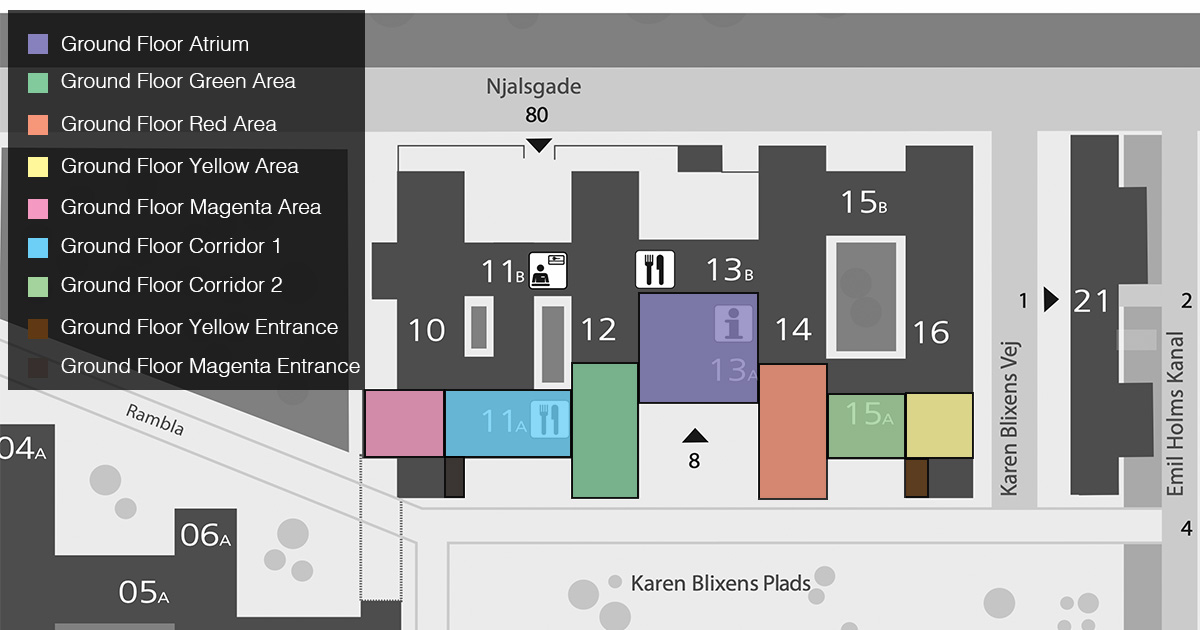
\includegraphics[width=\linewidth]{figures/map-ground-floor.jpg}
      \caption{Ground Floor}
      \label{fig:map-ground-floor}
    \end{subfigure}
    \hfill
    % subfigure
    \begin{subfigure}[b]{0.49\linewidth}
      \centering
      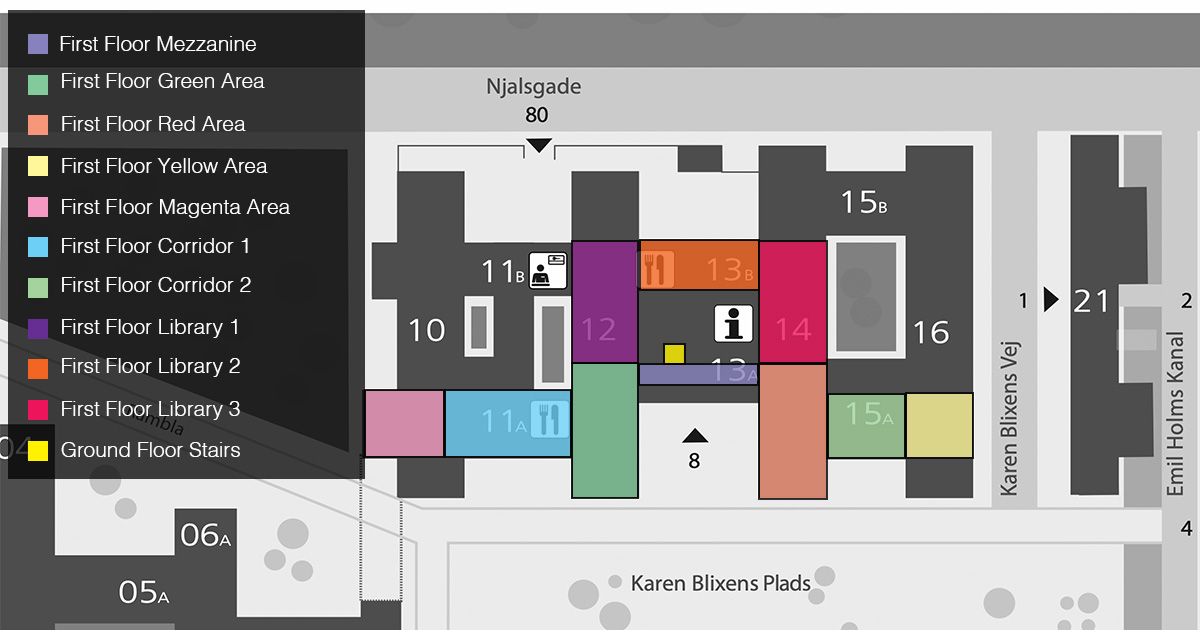
\includegraphics[width=\linewidth]{figures/map-first-floor.jpg}
      \caption{First Floor}
      \label{fig:map-first-floor}
    \end{subfigure}
    \caption{
      \textbf{Floor Plan of the Southern Campus of the Copenhagen with Location
      Labels.} The coloured regions represent the $|L|=20$ location labels as
      distributed over the two floors in the indoor space. It is apparent that
      a) the floor plan is similar across floors and b) that locations
      significantly differ in size.
    }
    \label{fig:map}
  \end{figure}

  
  % statistics of the data
  A total of $n=53$ videos of varying length were recorded, with an average
  duration of $\sim 57$s, amounting to a total number of $\sim 50$ minutes of
  footage, or an equivalent of $\sim 90K$ frames. Out of the total 53 videos
  that were recorded, 37 were used for training and 16 were used for testing.
  Importantly, the videos in the training split were recorded in a single
  session, while the videos in the test split were recorded on four separated
  days, in a span of two to four weeks after the training data had been
  recorded. This ensured that the trained model could be tested against unseen
  data, to more accurately assess its generalisation capabilities.

  % \begin{table}[ht]
  %   \centering
  %   \begin{tabular}{lccc}
  %   \toprule
  %    & Total Videos & Total Minutes & Total Frames \\
  %   \midrule
  %   Train & 37 &  37 & 67,200 \\
  %   Test  & 16 & 13 & 23,490 \\
  %   \midrule
  %   Total & \bfseries 53 & \bfseries 50 & \bfseries 90,690 \\
  %   \bottomrule
  %   \end{tabular}
  %   \caption{
  %     \textbf{Statistics of the Raw Data} The raw data consists of a total of 53
  %     videos, of which 37 were used for training and 16 for testing. The total
  %     duration of the raw data is 50 minutes, which amounts to a total of 90,690
  %     frames at a frame rate of 30 FPS.
  %   }
  %   \label{tab:raw-data}
  % \end{table}

  % TODO: figure about the time of data collection (side-by-side, one where hue
  %       denotes the split and the other where hue denotes the clips per day)

  % subsection data-collection (end)
  
  \subsection{Processed Data} % (fold)
  \label{sub:processed-data}

  A video classification models expects a single clip $c_i$ as input, which is a
  sequence of $s_v$ frames sampled from a video $v_i$ at a sampling rate $r_v$.
  . The number of frames per clip $s_v$ and the sampling rate $r_v$ are tied to
  the model architecture and are therefore fixed for each video classification
  model (Detail in Section~\ref{sub:models}). Clips are extracted in uniformly
  spaced intervals. This means that the number of clips $k_v$ that can be
  extracted from a video $v_i$ with $k$ frames is $\left\lfloor k / (r_v \cdot
  s_v) \right\rfloor$. The trailing frames that cannot be extracted as a clip
  are discarded. Each of the $k_v$ clips contains $s_v$ frames, leading to a
  total of $\left\lfloor k / (r_v \cdot s_v) \right\rfloor \cdot s_v$ frames for
  a single video. 

  Single-frame classification models expect a single frame $f_i$ from a video
  $v_i$ as input. Technically, all frames in a video $v_i$ could be used as
  input, but because of the strong local correlation between adjacent frames, it
  was hypothesised that models would overfit to the training data. For this
  reason, and in an attempt to make the training procedure more similar to the
  video classification models, a frame $f_i$ is sampled from a video $v_i$ at a
  sampling rate $r_f$. Here, $r_f$ is not tied to the model architecture and can
  be chosen freely. For all experiments $r_f$ was chosen to be $30$ for all
  single-frame classification, meaning only every 30th frame was sampled from a
  video. The number of frames $k_f$ that can be extracted from a video $v_i$
  with $k$ frames is $\left\lfloor k / r_f \right\rfloor$. It becomes clear that
  the frames considered per video $k_f$ is similar to the number of frames
  considered as part of clips if the two sampling rates $r_v$ and $r_f$ are
  equal, as

  \[
    \left\lfloor \frac{k}{r_v \cdot s_v} \right\rfloor \cdot s_v \approx
    \left\lfloor \frac{k}{r_f} \right\rfloor, \quad \text{if} \quad r_v = r_f
  \]

  The extraction of clips and frames for video and single-frame classification
  models, respectively, is illustrated in Figure~\ref{fig:data-extraction}. It
  shows that despite the same raw data source, the frames considered in the two
  datasets are not the same. This is because the frames in the video dataset are
  potentially sampled at a different rate than the frames in the single-frame
  dataset and because adjacent clips reset the sampling rate. However, it is
  hypothesised that due to large number of total frames and strong local
  correlation between adjacent frames, the two datasets are sufficiently similar
  to allow for comparison between the two model types.

  \begin{figure}[ht]
    \centering
    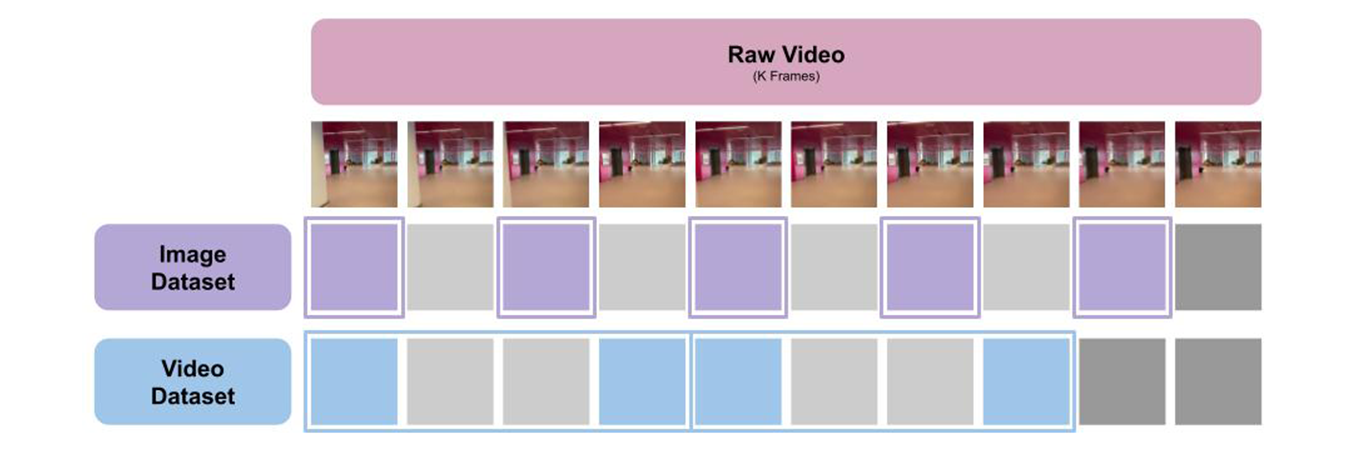
\includegraphics[width=0.95\textwidth]{figures/data-extraction.png}
    \caption{
      \textbf{Data Extraction.} A raw video with $k=10$ frames is processed into
      $k_f=5$ frames for the single-frame dataset and $k_v=2$ clips for the
      video dataset. Samples for each dataset type are indicated by a
      surrounding box. Frames are sampled at a rate of $r_f=2$ for the
      single-frame dataset and $r_v=3$ for the video dataset. A clip contains
      $s_v=2$ frames. Frames are colour-coded in correspondence to the dataset
      they belong to (single-frame dataset in purple and video dataset in blue),
      if they are sampled to the respective dataset. Discarded frames are
      coloured in grey (light-grey for within video frames, dark-grey for
      trailing frames).}
    \label{fig:data-extraction}
  \end{figure}
  
  Both image and video classification models expect a single sample $x_i$,
  whether it be a frame or a clip, to be standardised and of a certain size.
  Standardisation is performed on a per-channel basis after normalising the
  input to the range $[0, 1]$. Then, a sample $x_i$ is standardised as,

  \[
    x_{ic}' = \frac{x_{ic} - \mu_c}{\sigma_c} \quad \text{for} \quad c \in \{1, 2, 3\}
  \]

  , where $x_{ic}$ represents the channel $c$ of the sample $x_i$ and $x_{ic}'$
  is the standardised channel $c$ of the sample $x_i$. $\mu_c$ and $\sigma_c$ are
  taken from the ImageNet dataset~\cite{imagenet} for image classification
  models and from the Kinetics dataset~\cite{kinetics} for video 

  The height and width of each input frame is tied to the model architecture and
  is therefore fixed for each model. Input sizes are typically square and range
  from $182 \times 182$ to $224 \times 224$ for all models (Detail in
  Section~\ref{sub:models}). Resizing is performed in a non aspect-preserving
  manner to compress as much of the original viewport as possible into the
  resized frame. However, this also means that the trained models are likely to
  only perform well on frames with a similar raw aspect ratio as the training
  data (at least should be in portrait model).

  After all processing steps, the single-frame dataset contains $n_f$ samples
  and the video dataset contains $n_v$ samples. The number of samples $n_f$ and
  $n_v$ is dependent on the number of videos $n$ and the number of frames $k$ in
  each video. The final single-frame dataset can be written as $D_F = \{(f_1,
  y_1), ..., (f_{n_f}, y_{n_f})\}$, and the final video dataset as $D_V =
  \{(c_1, y_1), ..., (c_{n_v}, y_{n_v})\}$.

  % TODO: add statistics about nf and nv (number of frames and clips in train
  % and test)
  % TODO: mention that frames where sampled at a rate of 1FPS for train and
  % 30FPS for test

  % subsection data-preprocessing (end)


  \subsection{Models} % (fold)
  \label{sub:models}

  A deep learning model is supposed to learn a function $f: X \rightarrow Y$,
  where $X$ represents the input space and $Y$ the output space. In both
  single-frame and video classification, the output space is the discrete set of
  location labels, $Y = L = \{l_1, \ldots, l_n\}$. The input space $X$ is
  different for the two model types, as described in
  Section~\ref{sub:processed-data}. 

  A total of 10 different models are trained and evaluated in this work. The
  models are split into two categories: single-frame classification models and
  video classification models. The single-frame classification models are
  trained on the single-frame dataset $D_F$ and the video classification models
  on the video dataset $D_V$. A comprehensive overview of the models is given in
  Table~\ref{tab:model-overview}. The models are described in detail in the
  following.

  \begin{table}[ht]
    \centering
    \begin{tabular}{cllllllll}
      \toprule
      & \multirow{2}{*}{\textbf{Model}} 
      & \bfseries Release & \bfseries Rate & \bfseries F/C & \bfseries Size &
      \bfseries Params & \bfseries FLOPs & \bfseries Acc@1 \\
      & & (Y) & ($r_f$/$r_v$) & ($s_v$) & ($h$, $w$) & (M) & (G) & (\%) \\
      \midrule
    \multirow{9}{*}{\rotatebox[origin=c]{90}{Single-Frame}} 
    & AlexNet~\cite{alexnet} & 2012 & 30 & - & 224 & 61.1 & 0.71 & 56.52 \\
    & GoogLeNet~\cite{googlenet} & 2014 & 30 & - & 256 & 6.6 & 1.5 & 69.78 \\
    & ResNet18~\cite{resnet} & 2015 & 30 & -  & 224 & 11.7 & 1.82 & 82.52 \\
    & ResNet50~\cite{resnet} & 2015 & 30 & -  & 224 & 25.6 & 4.09 & 80.86 \\
    & DenseNet 121~\cite{densenet} & 2016 & 30 & - & 224  & 7.0 & 2.88 & 74.43 \\
    & MobileNet V3~\cite{mobilenetv3} & 2019 & 30 & - & 224  & 3.5 & 0.32 & 71.88 \\
    & ViT-B-16~\cite{vit} & 2020 & 30 & - & 224  & 86.7 & 17.56 & 81.07 \\
    & EfficientNet V2 S~\cite{efficientnetv2} & 2021 & 30 & - & 224  & 21.5 & 8.37 & 84.23 \\
    & ConvNext Tiny~\cite{convnext} & 2022 & 30 & - & 224  & 28.2 & 4.46 & 82.52 \\
    \midrule
    \multirow{2}{*}{\rotatebox[origin=c]{90}{Video}}
    & R(2+1)D~\cite{r2plus1d} & 2020 & 4 & 16 & 182 & 28.11 & 76.45 & 76.01 \\
    & X3D S~\cite{x3d} & 2020 & 6 & 13 & 3.5 & 182 & 2.96 & 73.33 \\
    \bottomrule
    \end{tabular}
    \caption{
      \textbf{Model Overview.} The table shows all models that were evaluated in
      this work. The models are split into two categories: single-frame models
      and video models. For each model, the table reports the release year
      (Release), the frame rate (Rate) of the training data, the number of
      frames per clip (F/C; \textit{only applicable to video classifiers}), the
      spatial resolution (Size) of the input images, the number of parameters in
      millions (Params), the number of floating point operations in billions
      (FLOPs) and the Top-1 accuracy (Acc\@1) on ImageNet~\cite{imagenet} for
      single-frame classification models and the top-1 accuracy on the
      Kinetics~\cite{kinetics} dataset for video classification models. The
      table is sorted by release date within each group.
    }
    \label{tab:model-overview}
  \end{table}

  \textbf{Alexnet} is a convolutional neural network that was introduced by
  Krizhevsky et al.~\cite{alexnet} in 2012. It was the first deep neural network
  to win the ImageNet Large Scale Visual Recognition Challenge~\cite{imagenet}
  and is considered to be one of the first successful application of deep
  learning to image classification. Architecturally, it uses the standard
  building blocks of convolutional nets. It consists of 5 convolutional layers
  (with filter sizes of $11 \times 11$, $5 \times 5$ and $3 \times 3$) with
  occasional max-pooling layers in between, followed by 3 fully connected
  layers. The network uses the ReLU activation function and dropout for
  regularization.

  \textbf{GoogLeNet} is a convolutional neural network that was introduced by
  Szegedy et al.~\cite{googlenet} in 2014. At its core, it is based on Inception
  modules, which allow the network to choose between multiple convolutional
  filter sizes in each block. Each inception module consists of 4 parallel
  convolutional layers, whose outputs are concatenated along the channel
  dimension. This advancement allowed the Google Team to significantly reduce
  the number of parameters in the network and win the ImageNet Large Scale
  Visual Recognition Challenge~\cite{imagenet} in 2014.

  \textbf{ResNet} was introduced by He et al.~\cite{resnet} in 2015. The main
  contribution of ResNet is the residual block, which allows the network to
  learn residual functions with respect to the layer inputs. This allows the
  network to be trained much deeper than previous architectures. The original
  ResNet paper introduced several architectures with different depths. In this
  work, we use ResNet18 and ResNet50, which are among the smallest architectures
  in the family.

  \textbf{Densenet} was introduced by Huang et al.~\cite{densenet} in 2016. The
  main contribution of Densenet is the dense block, which allows the network to
  learn feature maps from all preceding layers. This allows the network to be
  trained much deeper than previous architectures. The original Densenet paper
  introduced several architectures with different depths. In this work, we use
  Densenet121, which is among the smallest architectures in the family.

  \textbf{MobileNet V3} was introduced by Howard et al.~\cite{mobilenetv3} in
  2019. The main contribution of MobileNet V3 is the efficient inverted
  bottleneck block.

  \textbf{ViT} was introduced by Dosovitskiy et al.~\cite{vit} in 2020. It is
  the first attempt to apply the Transformer architecture proposed by Vaswani
  et. al~\cite{transformer} to computer vision task. The main contribution of
  ViT is the patch embedding mechanism, which allows to transform a
  two-dimensional image into a one-dimensional sequence of tokens that,
  alongside a positional encoding, can be processed by the Transformer
  architecture. The original ViT paper introduced several architectures with
  different depths. In this work, we use ViT-B-16, which uses a patch dimension
  of $16 \times 16$.

  \textbf{EfficientNet V2} was introduced by Tan et al.~\cite{efficientnetv2} in
  2021.The main contribution of EfficientNet V2 is the efficient inverted
  bottleneck block, that also underlies MobileNet V3~\cite{mobilenetv3}.

  \textbf{ConvNext} is the most recent model in this work. It was introduced by
  Wang et al.~\cite{convnext} in 2021, producing state-of-the-art results.

  \textbf{R(2+1)D} was introduced by Tran et al.~\cite{r2plus1d} in 2018. It is
  the first attempt to apply the ResNet architecture~\cite{resnet} to video
  classification tasks. The main contribution of R(2+1)D is the spatiotemporal
  convolutional block, which allows the network to learn spatiotemporal
  features. The original R(2+1)D paper introduced several architectures with
  different depths. In this work, we use R(2+1)D-18.

  \textbf{X3D} was introduced by Feichtenhofer et al.~\cite{x3d} in 2020.
  \textit{TBD}.

  % subsection models (end)

  \subsection{Training} % (fold)
  \label{sub:training}

  All models were implemented using the PyTorch framework~\cite{pytorch} and the
  training was performed remotely on the high performance cluster (HPC) of the
  IT University of Copenhagen. The HPC consists of multiple computing nodes. For
  this training, a single node was used with GPU acceleration. For more details
  on the hardware specifications see the Appendix (Section~\ref{sec:appendix}).

  During training, all models were evaluated using the standard multi-class loss
  function cross-entropy loss (Equation~\ref{eq:cross-entropy}), which is
  defined as,

  \begin{equation}
    \mathcal{L}(\hat{\mathbf{y}},\mathbf{y}) = -\sum_{i=1}^{L} \mathbf{y}_i
    \log(\hat{\mathbf{y}}_i) \quad .
    \label{eq:cross-entropy}
  \end{equation}

  % TODO: compare to pytorch cross-entropy loss (is it the same? what is the
  % difference to nll?)

  Here, $\hat{\mathbf{y}}$ is the predicted probability distribution over the $L$
  location labels and $\mathbf{y}$ is the one-hot encoded ground truth location
  label. 

  All models were trained using the AdamW~\cite{adamw} optimiser with default
  parameters, except for the learning rate, which was set to a constant of
  $1e^{-4}$. The batch size was set to 32 for all image classifiers and 4 for
  all video classifiers due to memory limitations. Unless otherwise specified,
  all image and video classifiers were trained with the same set of training
  hyper-parameters, which are specified in Table \ref{tab:default-hyperparams}. 

  \begin{table}[ht]
    \centering
    \begin{tabular}{rllll}
      \toprule
      Classifier & Batch Size & Epochs & Optimiser & Learning Rate Scheduler \\
      \midrule
      \bfseries Image & 32 & 10 & AdamW ($\gamma=1e^{-4}$) & Step-LR
      ($\gamma=1e^{-1}, s=5$) \\
      \bfseries Video & 8 & 10 & AdamW ($\gamma=1e^{-4}$) & Step-LR
      ($\gamma=1e^{-1}, s=5$) \\
      \bottomrule
    \end{tabular}
    \caption{Default Hyperparameters for Image and Video Classifiers}
    \label{tab:default-hyperparams}
  \end{table}

  %   (end)

  \subsection{Evaluation} % (fold)
  \label{sub:evaluation}

  To assess all models in terms of their performance and efficiency on the task
  of location classification, a series of different performance and efficiency
  metrics are computed. All metrics are computed on the test set, which was
  separated from the original dataset before training, as described in
  Section~\ref{sub:raw-data}.

  The accuracy of the models is evaluated using the standard multi-class top-1
  and top-3 accuracy metric. It is the ratio of samples, for which the correct
  label is among the top-1 or top-3 predictions, respectively. As some location
  labels are naturally underrepresented in the dataset due to the natural
  variation in size of the different locations, the macro F1-score is used to
  compute a more fine-grained metric that gives more weight to
  resource-constrained locations. The macro F1-score is the average of the
  class-specific F1-scores, which are defined as the harmonic mean of precision
  $P_i$ and recall $R_i$. All performance metrics where computed using the
  TorchEval library~\textit{[CITE]}.

  To assess the efficiency of the models a series of benchmarks were performed
  on the HPC. The benchmarks were performed using the \texttt{PyTorch Benchmark}
  library~\textit{pytorch-benchmark}. The library allows to track various
  metrics during unbatched and batched inference. Results are aggregated over 5
  passes and the mean and standard deviation are reported. Out of all computed
  metrics, the mean inference time per sample (latency) and mean number of
  samples per second (throughput) were further considered.

  Due to different nature of the underlying datasets $D_f$ and $D_v$, the
  performance and efficiency metrics are not directly transferable. For example,
  the top-1 accuracy of the image classifiers is the number of correctly
  predicted frames, whereas the top-1 accuracy of the video classifiers is the
  number of correctly predicted videos. While this limits the comparability of
  the metrics, it is still possible to draw conclusion between the different
  model types due to the relatively large number of samples and the natural
  resemblance of frames and clips.

  To analyse the model behaviour in more detail, the models were also evaluated
  qualitatively by manually inspecting the confusion matrix and a subset of the
  misclassified samples for the best-performing single-frame and video
  classification model. 

  % Furthermore, the \texttt{GradCam}~\cite{gradcam} algorithm was used to gain
  % insights into the internal functioning of the model. GradCam is a technique
  % that backtracks the activations in the convolutional filters of the model at
  % some depth in the model's architecture and through the gradients of the model
  % to the input image. This allows to visualise the regions of the image that
  % were most relevant for the model to make its prediction. In this scenario, it
  % is hoped that the highlighted regions can be used to understand what types of
  % features the model is looking for in the image and what types of features it
  % is not looking for. This can be used to identify potential issues with the
  % model and to gain insights into how the model can be improved.

  % subsection evaluation (end)

  % section methodology (end)

  \section{Results} % (fold)
  \label{sec:results}

  % computer vision models are capable of solving indoor localisation when
  % phrased as a classification task

  We show that computer vision models, when carefully designed and trained, are
  generally capable of solving the task of indoor localisation when phrased as a
  coarse-grained classification problem. The results of the evaluation are
  presented in Table~\ref{tab:results}.

  \begin{table}[ht]
    \begin{tabular}{cllll|llll}
    \toprule
    & \multirow{2}{*}{\textbf{Model}} 
    & \bfseries Acc@1 & \bfseries Acc@3 & \bfseries Ma.-F1 & \bfseries FLOPs &
      \bfseries Latency & \bfseries Throughput \\
    & & (\%) & (\%) & (\%) & (G) & (ms/Pred) & (Preds/s) \\
    \midrule
    \multirow{8}{*}{\rotatebox[origin=c]{90}{Single Frame}}
    & AlexNet & 56.67 & 81.36 & 50.79 & 0.71 & 14.1 & 70.91 \\
    & Google LeNet & 63.40 & 84.74 & 56.80 & 1.97 & 47.2& 21.17 \\
    & DenseNet121 & 67.79 & 83.04 & 63.05 & 2.88 & 71.9 & 13.89 \\
    & ResNet18 & 70.65 & 89.73 & 64.84 & 1.82 & 27.1 & 37.22 \\
    & ResNet 50 & 55.76 & 77.65 & 50.05 & 4.12 & 60.9 & 16.41 \\
    & MobileNet V3 Small & 28.68 & 51.34 & 19.21 & 0.06 & \bfseries 11.9 & \bfseries 83.82 \\
    & ViT B-16 & 53.20 & 77.57 & 47.54 & 17.59 & 166.0 & 6.03 \\
    & EfficientNet V2 Small & 50.51 & 81.73 & 41.71 & 2.88 & 77.6 & 12.91 \\
    \midrule
    \multirow{2}{*}{\rotatebox[origin=c]{90}{Video}}
    & R(2+1)D & \bfseries 78.33 & \bfseries 91.67 & \bfseries 75.27 & \bfseries 93.72 & 825.1 & 1.22 \\
    & X3D & 68.89 & 81.11 & 54.09 & 2.85 & 229.0 & 4.37 \\
    \bottomrule
    \end{tabular}

    \caption{ 
      \textbf{Results.} The table the performance and efficiency metrics for all
      trained models. The models are grouped by their type (single-frame or
      video). The performance metrics are the top-1 accuracy (Acc@1), top-3
      accuracy (Acc@3) and Macro F1-Score (Ma.-F1). The efficiency metrics are
      the number of floating point operations (FLOPs) per inference, the mean
      inference time in milliseconds per prediction (Latency) and the mean
      number of predictions per second (Throughput). The best performing model
      in each category is highlighted in bold. The metrics are computed on the
      test set of the respective dataset. 
    }
    \label{tab:results} 
  \end{table}

  \subsection{Detailed Analysis of Single-Frame Classifiers} % (fold)
  \label{sub:analysis-single-frame-classifiers}

  % single-frame classifiers are capable of solving the task
  Surprisingly, even simple single-frame classification models are capable of
  providing a reasonable solution to the task of indoor localisation. Despite
  the lack of information about the temporal context of the frames, the
  best-performing single-frame classifier (ResNet18) achieves a top-1 accuracy
  of 70.65\% and a top-3 accuracy of 89.73\%. This is a significant result as it
  shows that processing single frames of the video is sufficient to solve the
  task of indoor localisation. This is especially important in the context of
  mobile devices, and application where live inference is required.

  % single-frame classifiers are efficient
  Out of the single-frame classifiers, three classifiers can produce real-time
  predictions on a mobile device, as the have a higher throughput rate than
  video frame rate. The most efficient model is MobileNet V3 with a throughput of
  83.82 predictions per second. AlexNet and ResNet18 are also capable of
  real-time inference with throughputs of 70.91 and 37.22 predictions per
  second, respectively. All other models are not capable of real-time inference
  on a mobile device, but are sufficiently quick to provide near real-time
  predictions.

  % model complexity vs. performance
  Evidence in computer vision research suggests that more complex models
  typically are able to achieve better performance. This is not entirely the
  case for this study. The smallest model, MobileNet V3, is a clear outlier in
  terms of performance, only achieving a top-1 accuracy of 28.68\%. It is
  hypothesised that the model is not complex enough to handle the challenging
  20-class classification task.

  Performance steadily increases with the number of parameters up to the
  complexity of ResNet18 (11.2M), but then decreases again. Interestingly, the
  most complex model in terms of the total number of parameters, ViT-B-16
  (85.8M), which achieves state-of-the-art results on common image
  classification benchmarks, is not the best-performing model in this study.
  This is likely due to the small size of the dataset in combination with
  relatively few training epochs. 

  % end subsection analysis-single-frame-classifiers

  \subsection{Detailed Analysis of Video Classifiers} % (fold)
  \label{sub:detailed-analysis-of-video-classifiers}

  As the nature of the task is inherently temporal, it is not surprising that
  video classifiers outperform single-frame classifiers
  (Figure~\ref{fig:performance-metrics}). The best performing video classifier is
  R(2+1)D with a top-1 accuracy of 78.33\% and a top-3 accuracy of 91.67\%. This
  is a significant improvement over the best performing single-frame classifier,
  ResNet18. The video classifiers are more robust to noise in the input data, as
  they are able to leverage the temporal context of the video. For example, the
  model is capable of predicting a clip correctly despite a few frames being
  occluded by a person walking through the scene or other sources of noise. This
  capability has proven especially useful in the context of indoor localisation,
  as high variation in the environment and therefore high noise in the input
  data is common.

  % video classifiers are less efficient
  Video classifiers generally require more compute and memory resources during
  inference, as they have to keep a history of the previous frames in memory.
  This is reflected in the efficiency metrics. R2+1D has a throughput of only
  1.22 predictions per second. This means that it can only provide predictions
  for the location every second. This makes the model slower in responding to
  sudden changes in the environment.

  % subsection detailed analysis of video classifiers (end)

  \begin{figure}
    \begin{center}
      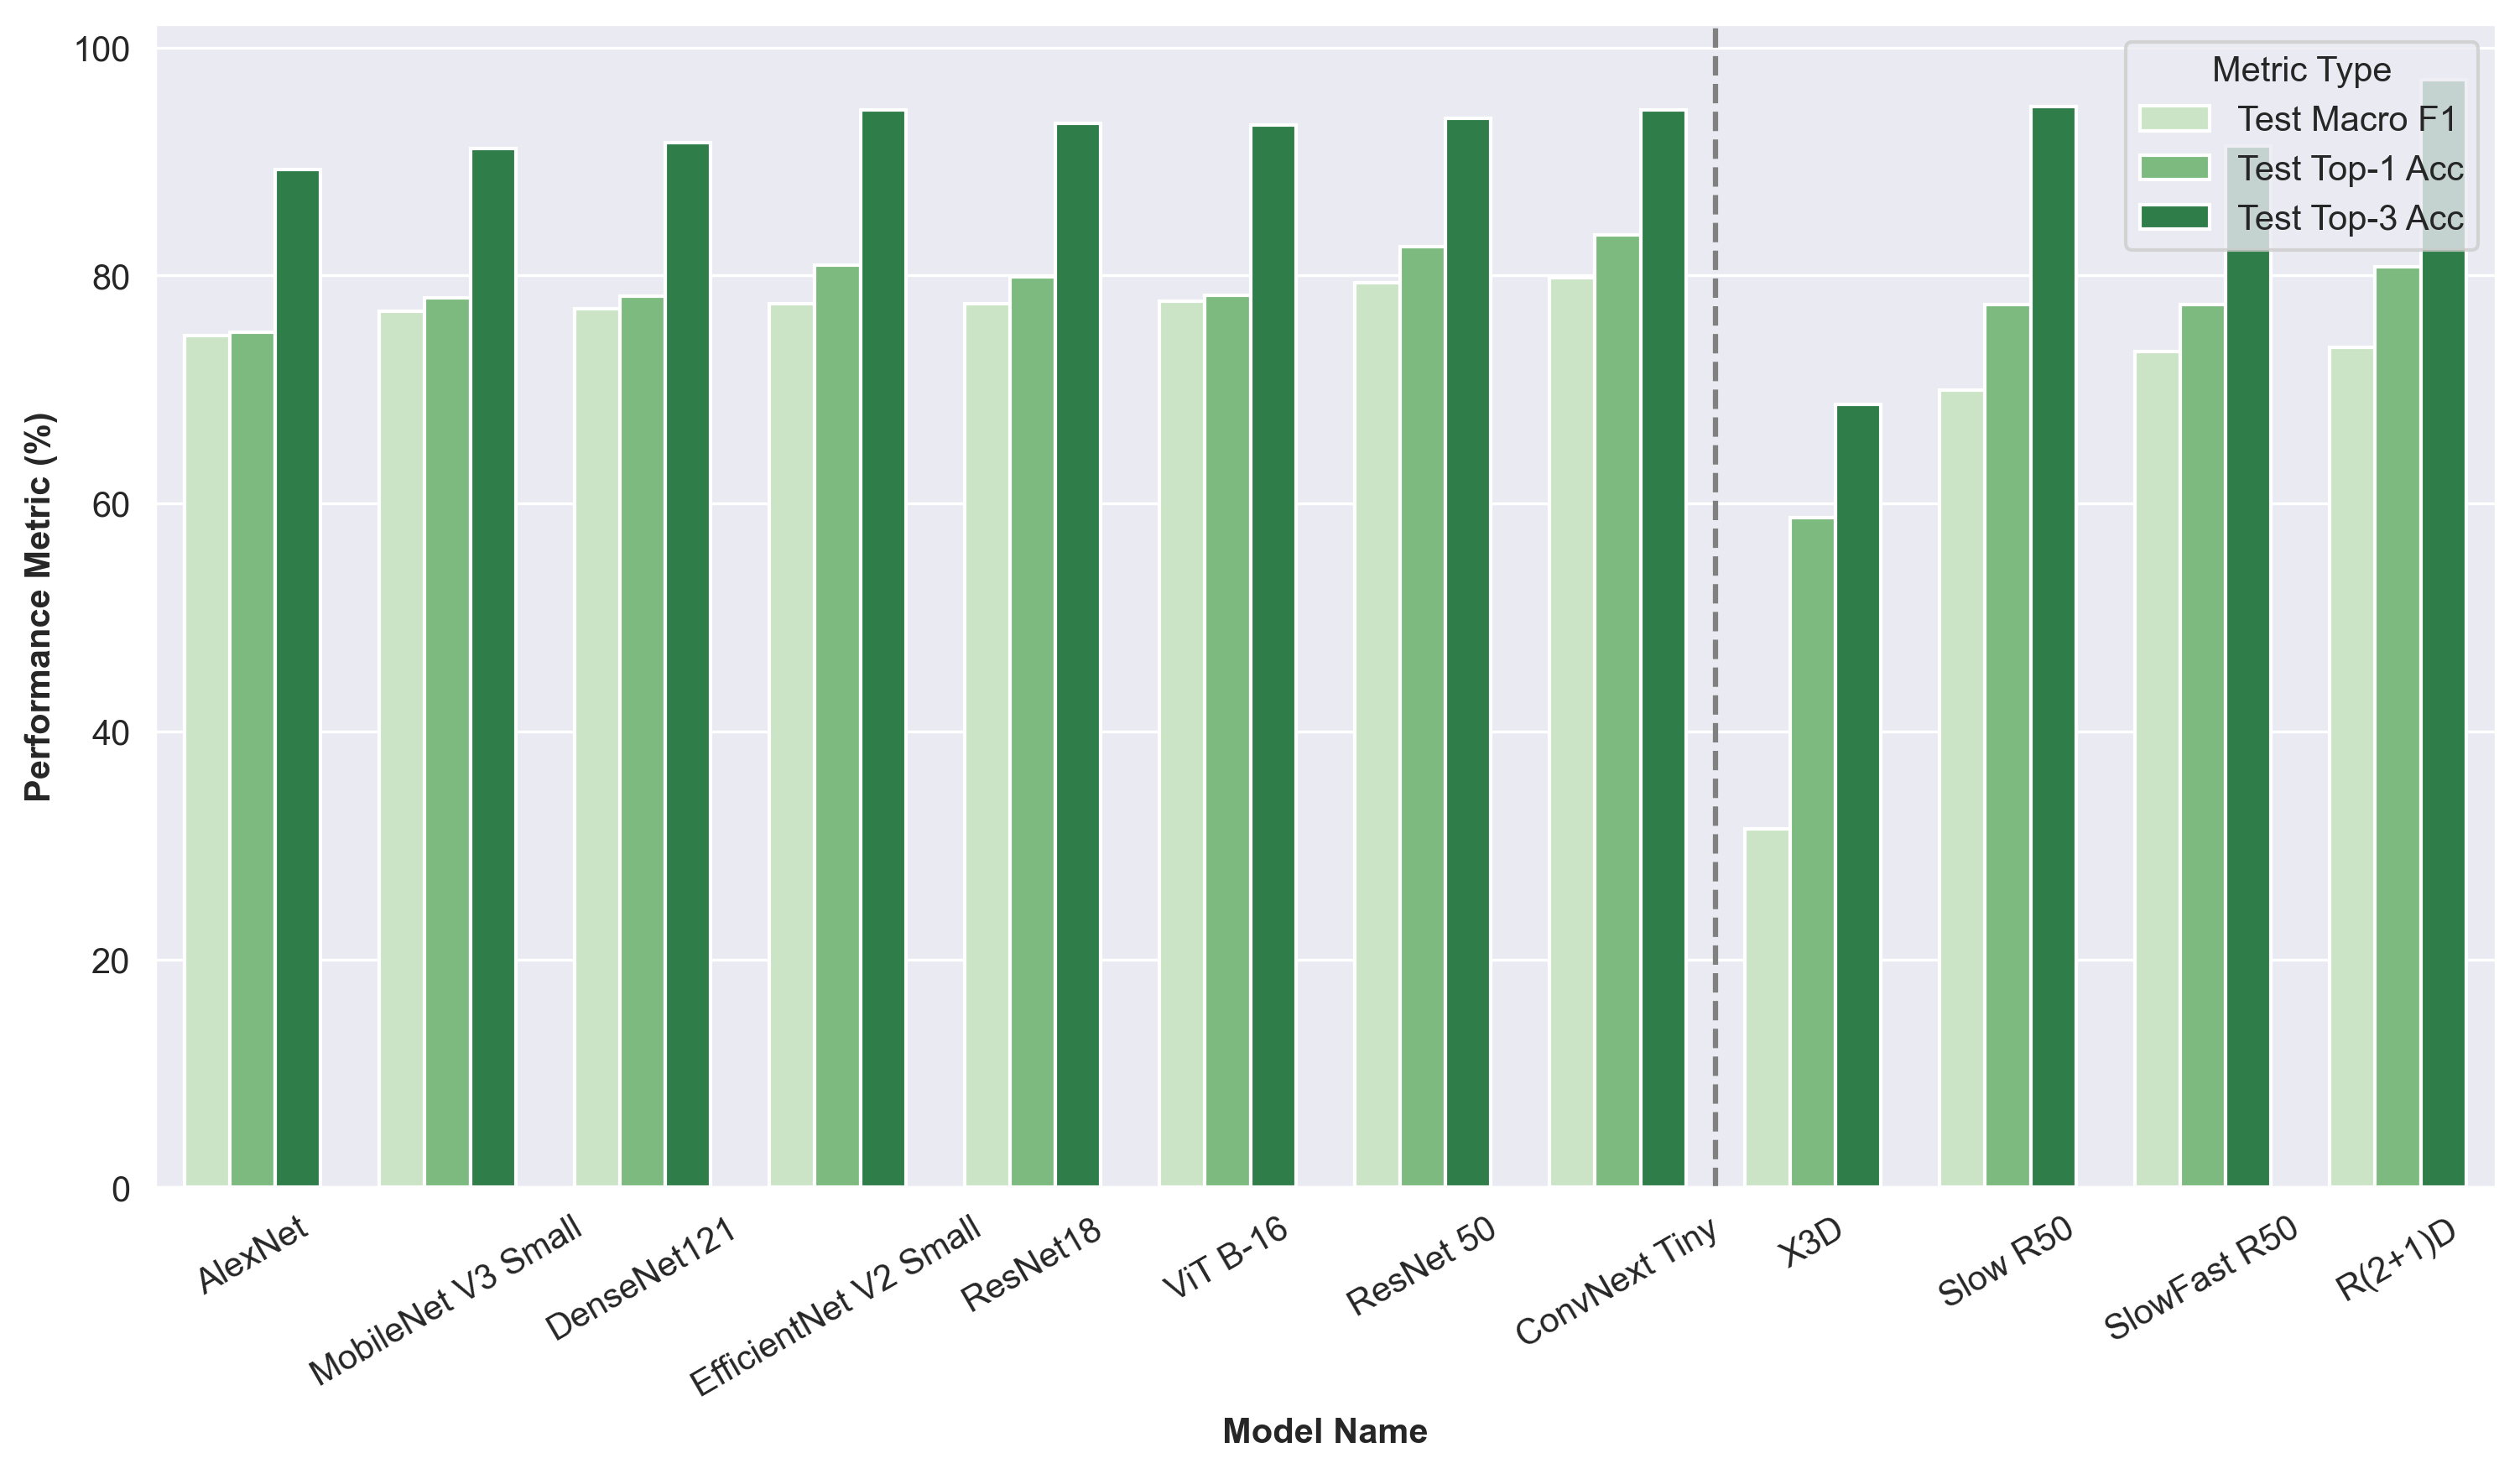
\includegraphics[width=.95\textwidth]
      {./figures/performance-metrics.png}
    \end{center}

    \caption{\textbf{Performance Metrics.} The Figure shows the performance
      metrics, Macro F1, Top-1 Accuracy and Top-3 Accuracy, for all trained
      models on the test split. A grey, dotted line separates the single-frame
      classifiers (left) from the video classifiers (right). Within their group,
      models are sorted from left to right by their Top-1 Accuracy.}

    \label{fig:performance-metrics}
  \end{figure}

  \subsection{Performance Efficiency Trade-Off} % (fold)
  \label{sub:tradeoff}

  The pre-dominant tendency in deep learning is that with sufficient data sizes
  and compute resources, more complex models outperform simpler ones. However,
  there is a trade-off between model complexity and efficiency, when inference
  time is critical like when deployed on a mobile device. 

  Figure~\ref{fig:tradeoff} shows the Top-1 Test Accuracy of all models against
  latency (left) and throughput (right). Latency and throughput are meaningful
  metrics to assess model's efficiency, as they are a direct proxy for the
  real-time inference speed when deployed on low-resource device. While the
  benchmarks were computed on a desktop CPU, they give a good indication of the
  relative performance of the models and allow to extrapolate the insights to
  performance on a mobile device. It is to be noted that latency and throughput
  are inversely proportional to each other: Less inference time per sample (low
  latency) leads to a higher number of inferences per second (high throughput).
  However, as inference times vary greatly between models, the two metrics are
  plotted separately, as they highlight different tails of the distribution.
  Specifically, the latency plot accentuates high latency models, while the
  throughput plot highlights low latency models.

  % latency-accuracy
  In Figure~\ref{fig:tradeoff}a, R(2+1)D is a clear outlier. The model has the
  highest latency, but also the best overall performance. The increase in
  complexity over X3D seems to be justified, as the model achieves a 9.4\%
  increase in Top-1 Accuracy, while only increasing the latency by 0.6 seconds.
  A similar trend cannot be observed for the single-frame classifiers. As
  latency times are close to each, their trend is easier to study in
  Figure~\ref{fig:tradeoff}b. Here, a quadratic relationship between throughput
  and accuracy can be observed for the single-frame classifiers.
  High-complexity, but low-throughput models, like ViT-B-16, EfficientNet V2 S
  and ResNet18 are outperformed by lower-complexity models. Similarly,
  low-complexity, but high-throughput models, like MobileNet V3 and AlexNet,
  show similarly low performance. The sweet spot in terms of throughput and
  accuracy is ResNet18, which achieves a throughput of 37.22 predictions per
  second and a top-1 accuracy of 72.92\% This phenomenon is best explained by
  the fact that low-complexity models are not able to capture the complexity of
  the task, while high-complexity models are not able to learn from the small
  dataset. The video classification models defy this trend, as they are all
  low-throughput, but high-performing.

  \begin{figure}
    \centering
    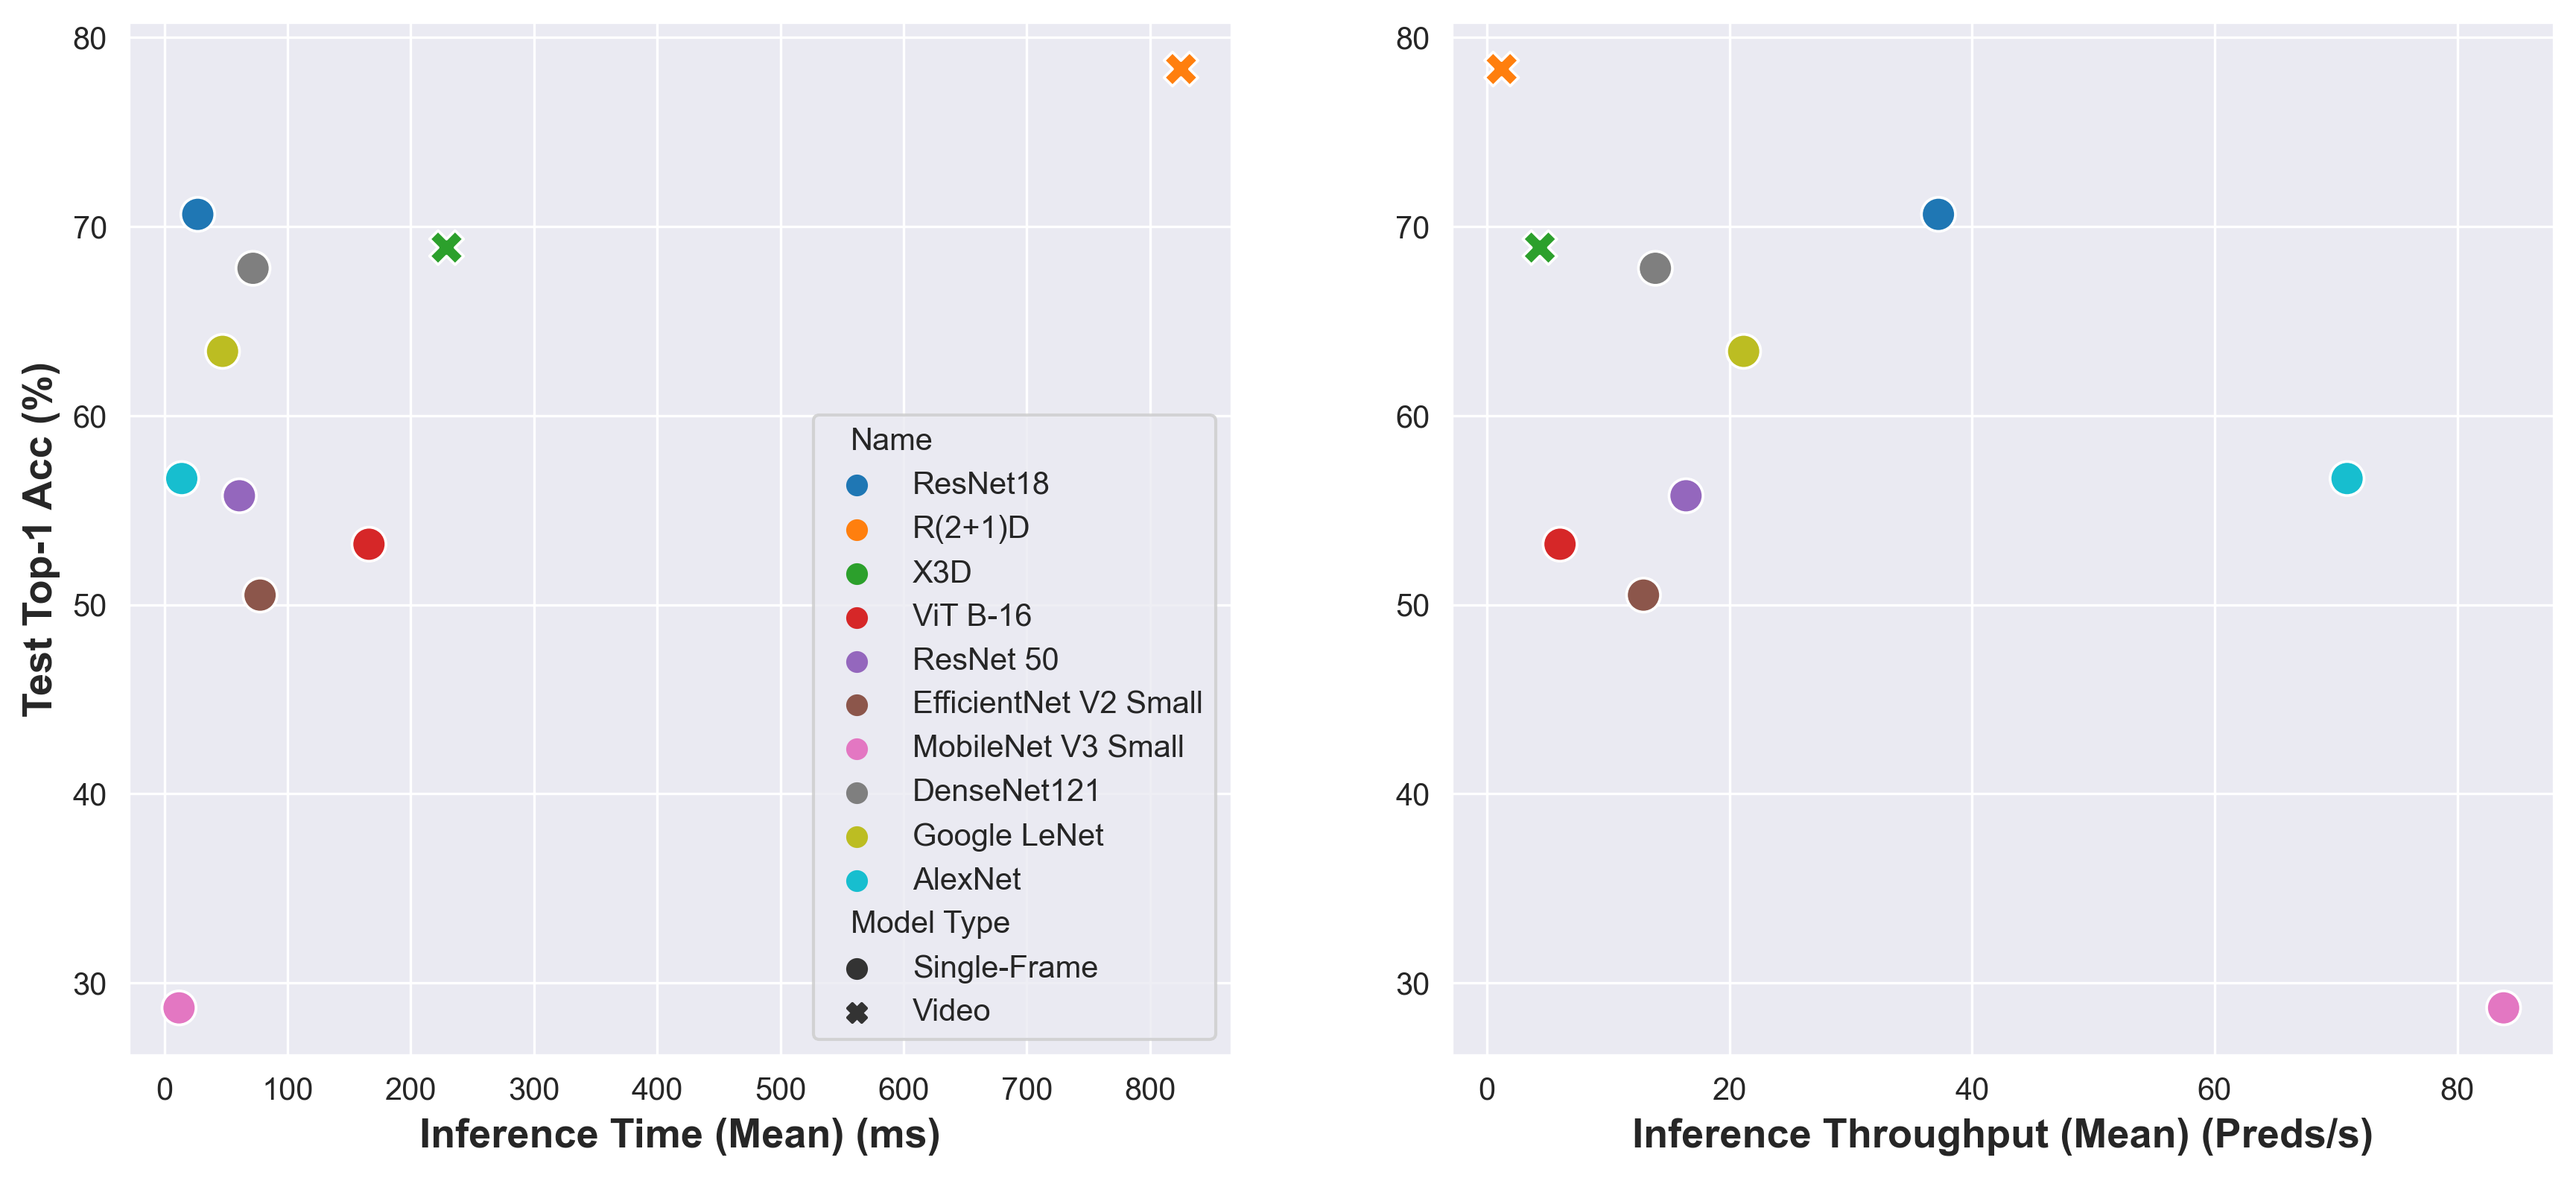
\includegraphics[width=\textwidth]{
    ./figures/performance-efficiency-tradeoff-scatter.png}
    \caption{
      \textbf{Performance-Efficiency Trade-Off.} The Figure visualises the
      performance-efficiency trade-off for all models by plotting the
      relationship between the Top-1 Accuracy against the latency (inference
      time in milliseconds per prediction) and throughput (predictions per
      second). Each model is given unique colour, and the marker type indicates
      whether the model is a single-frame classifier (circle) or a video
      classifier (cross).
    }

    \label{fig:tradeoff}
  \end{figure}

  % subsection tradeoff (end)

  \subsection{Analysing Prediction Patterns: Confusion Matrices} % (fold)
  \label{sub:conf-matrices}
  
  To better understand the strengths and weaknesses of deep learning models in
  tackling the task of indoor classification, the two best performing models,
  ResNet18 and R(2+1)D, are analysed in more detail. Specifically, the confusion
  matrices of the two models are analysed to identify common failure modes of
  the models.

  Figure~\ref{fig:conf-matrix} shows the confusion matrices for (a) ResNet18 and
  (b) R(2+1)D. It becomes clear that both models struggle with the same
  misclassification scenarios. The most common misclassification is between the
  two corridors on the ground floor (\textit{Ground Floor Corridor 1} and
  \textit{Ground Floor Corridor 2}) and the Atrium (bottom-right grey
  rectangle). ResNet18 both confuses the two corridors and has a tendency for
  predicting the majority class (Atrium) instead of Corridor 2. R(2+1)D rarely
  confuses the corridor, but has an even stronger tendency for predicting
  Corridor 2 as Atrium. These failure cases are explained by the fact that the
  two corridors and the Atrium are visually very similar. Furthermore, they are
  directly adjacent to each other, which likely leads to some naturally
  occurring failure cases at the border of the areas. Here, the model might
  predict the new class earlier or later than the ground truth label changes.

  Another region with similar behaviour are the three libraries on the first
  floor (\textit{First Floor Library}, \textit{First
  Floor Library 2}, \textit{First Floor Library 3}). Especially ResNet18
  struggles to distinguish between the three classes, which is understandable
  given the fact that the dominating visual feature of the three classes are 
  rows of bookshelves. R(2+1)D shows a similar, but less pronounced behaviour.
  One explanation might be that while the shared visual feature of bookshelves,
  the arrangement of the bookshelves is different in the three libraries, which
  can be learned by R(2+1)D due to its temporal modelling capabilities.

  \begin{figure}
    \centering
    \begin{subfigure}[b]{0.49\textwidth}
      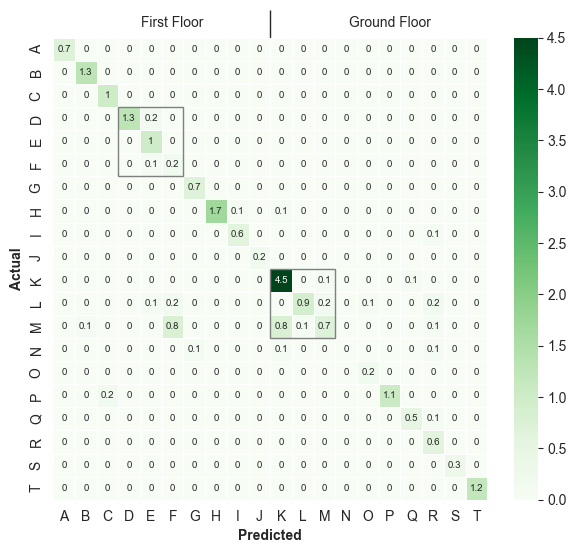
\includegraphics[width=\textwidth]{./figures/conf-matrix-resnet18.png}
      \caption{ResNet18}
    \end{subfigure}
    \begin{subfigure}[b]{0.49\textwidth}
      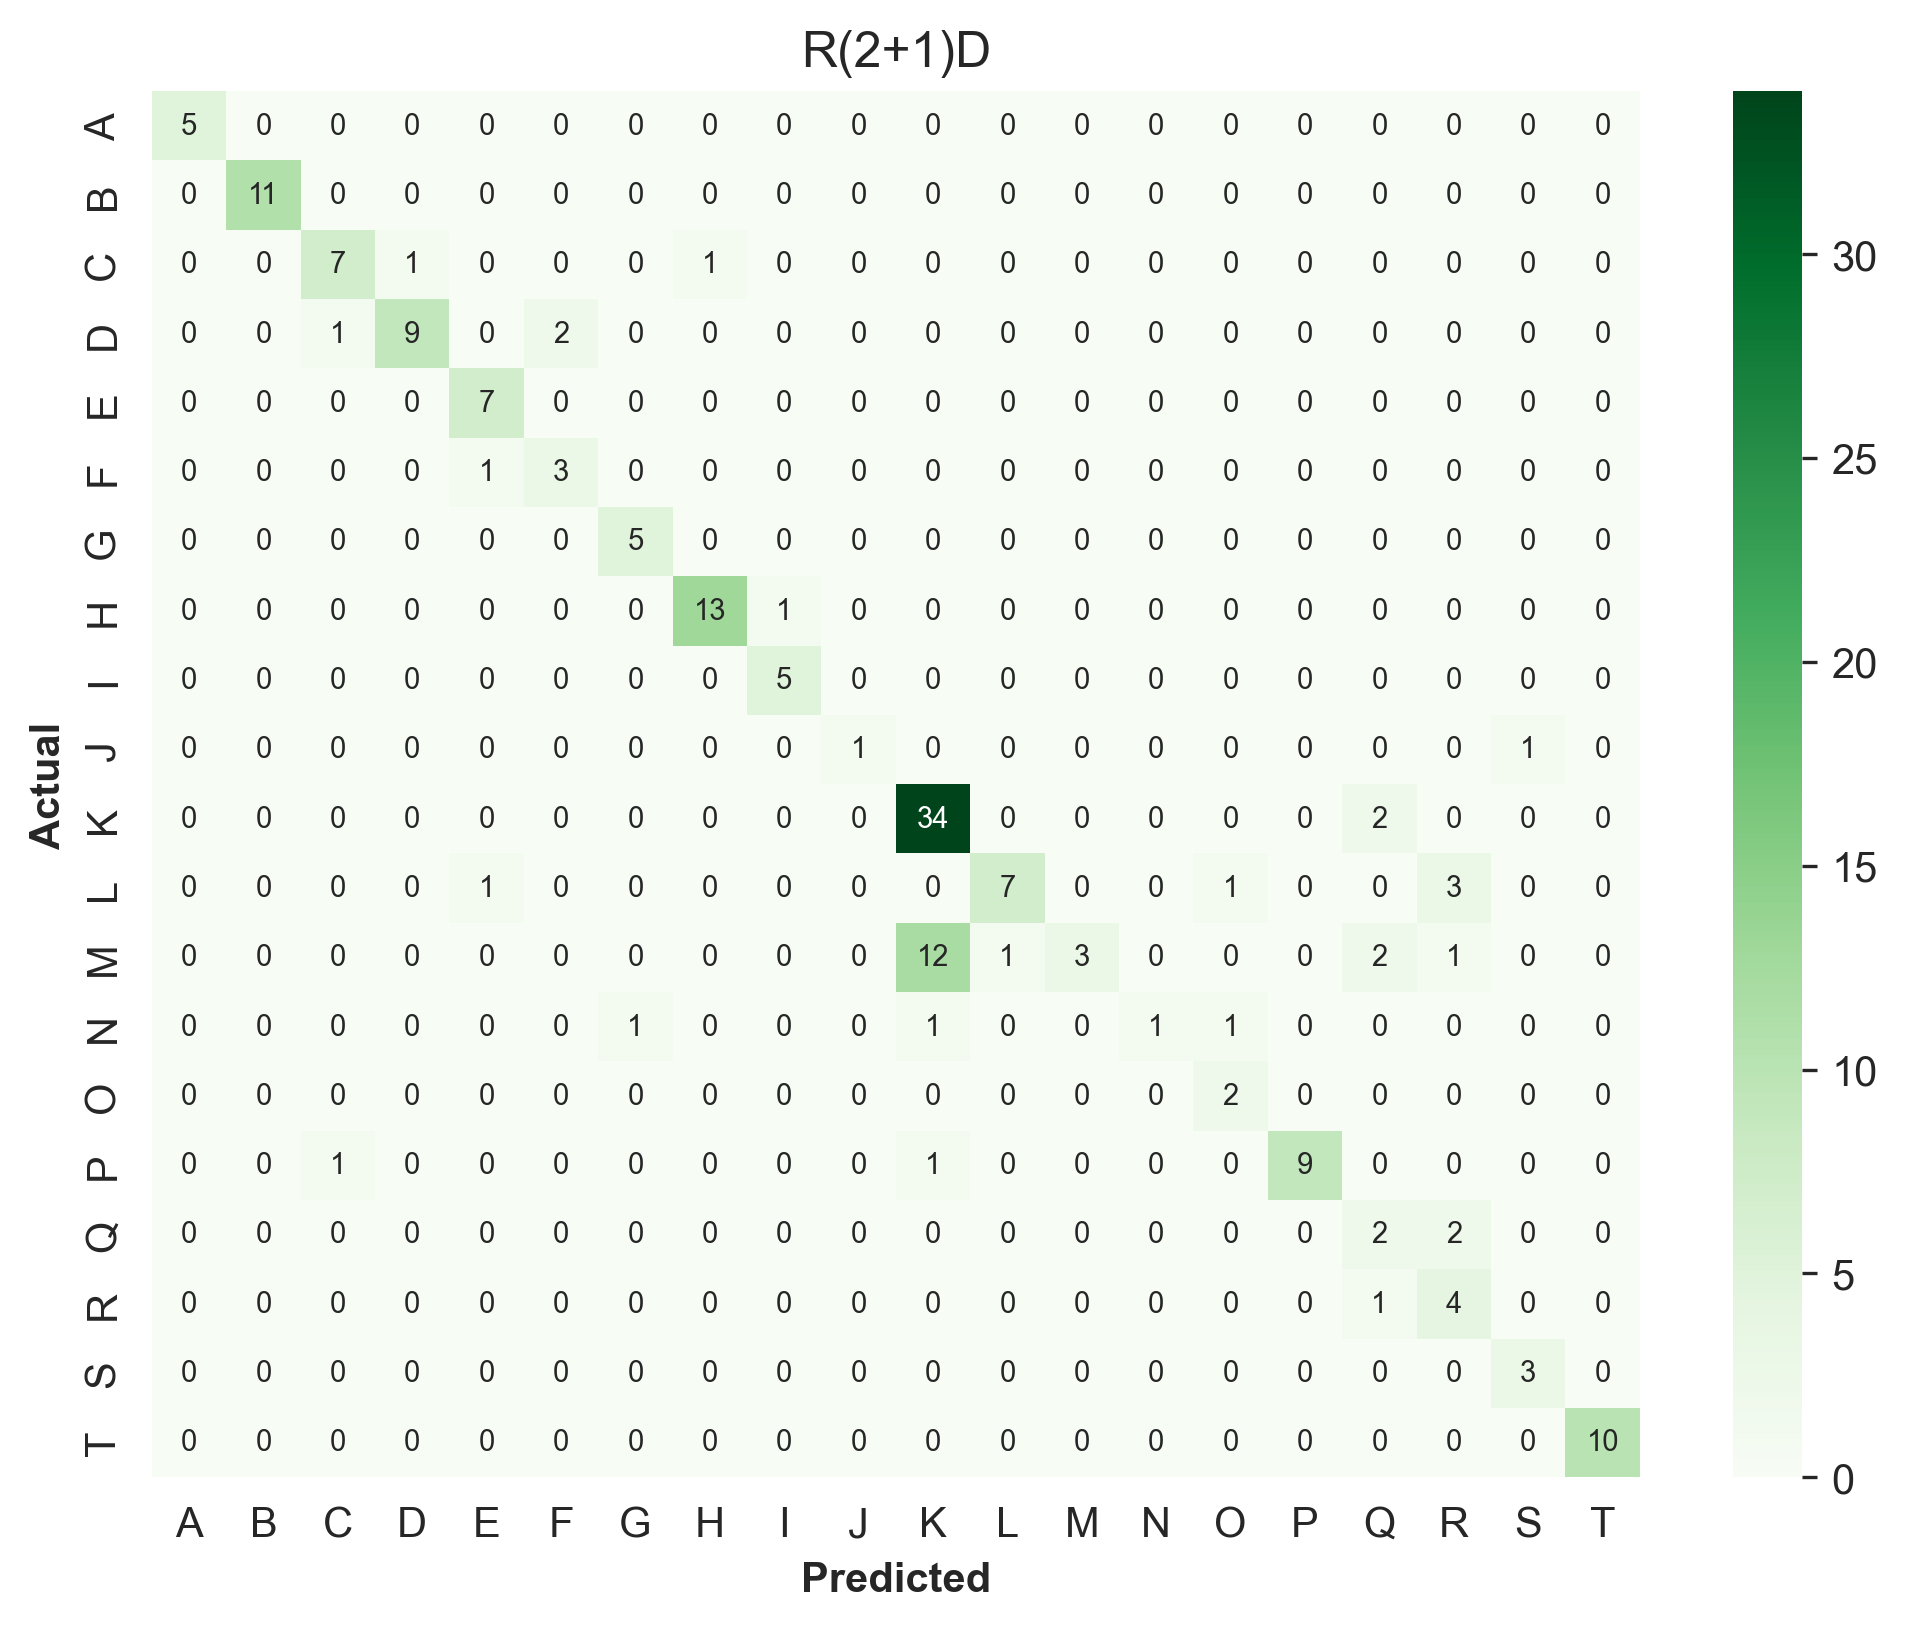
\includegraphics[width=\textwidth]{./figures/conf-matrix-r(2+1)d.png}
      \caption{R(2+1)D}
    \end{subfigure}
    \caption{
      \textbf{Confusion Matrices.} The Figure shows the confusion matrix for (a)
      ResNet18 (best performing single-frame classifier) and (b) R(2+1)D (best
      performing video classifier). The confusion matrix of ResNet18 is
      normalised to show 1K samples per class for visual purposes. For both
      matrices, the entry at row $i$ and column $j$ shows the number of samples
      that belong to class $i$ but were predicted to be class $j$. Gray
      rectangles indicate challenging classes, that are often confused.
    }
    \label{fig:conf-matrix}
  \end{figure}

  % TODO: add conf matrices with classes ordered by ground/ first floor
  % similarity

  \subsection{Analysing Failing Scenarios: Mispredicted Samples} % (fold)
  \label{sub:mispredicted}

  Figure~\ref{fig:mispredicted} shows three exemplary mispredicted samples for
  (a) ResNet18 and (b) R(2+1)D. The respective legend shows the top 3 predicted
  classes for each sample in order of confidence and the ground truth label. 

  For ResNet18, the first sample shows a misclassification between the two
  corridors on the ground floor, which is the most common misclassification for
  ResNet18 as seen from the confusion matrix (Figure~\ref{fig:conf-matrix}a). It
  can be seen, that the model is unsure about the prediction (64\% confidence in
  Corridor 2 and 34\% confidence in Corridor 1). The second and third sample
  show another common misclassification mode. Here the model confuses the 
  the yellow and green area on the ground and first floor, respectively.

  For R(2+1)D, the first sample shows a transition misprediction. The frame is
  directly at the border between the Magenta Area and Corridor 2 on the ground
  floor and predicts the Magenta Area, while the ground truth label is Corridor
  2. The second sample shows a truly sample from a challenging video from the
  test split, because the video shows an area that was freshly painted in blue
  in Corridor 2. As the training split does not contain any videos from this
  area, the model has never seen this area in blue and thus predicts a wrong
  area, in this case the majority class Atrium. The third sample shows another 
  misprediction of similar classes. The clip starts at the very end of the
  entrance with the camera facing to the outside. The model predicts the yellow
  entrance, when the ground truth label is the magenta entrance.


  \begin{figure}
      \centering
    \begin{subfigure}[b]{\textwidth}
      \centering
      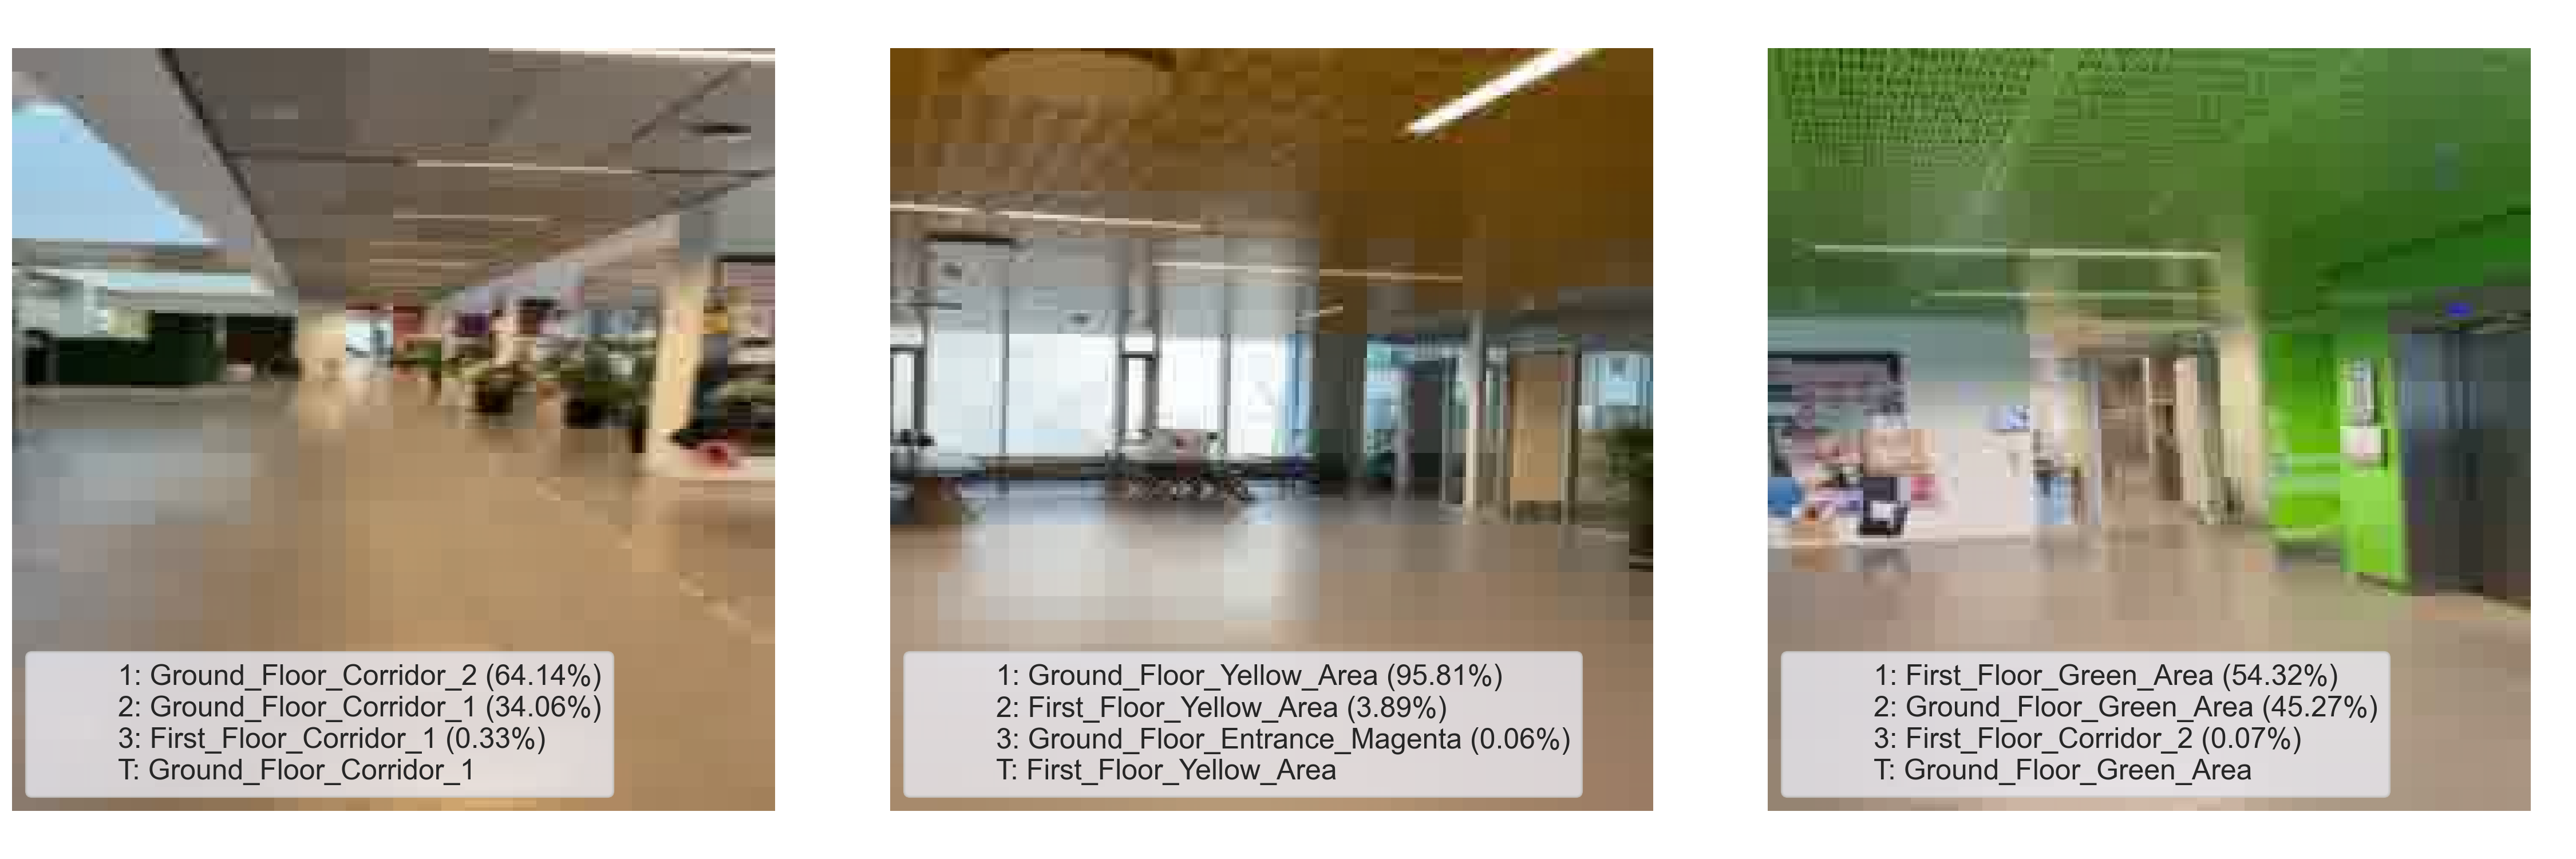
\includegraphics[width=\textwidth]{./figures/resnet18-mispredicted-frames.png}
      \caption{ResNet18}
    \end{subfigure}
    \begin{subfigure}[b]{\textwidth}
      \centering
      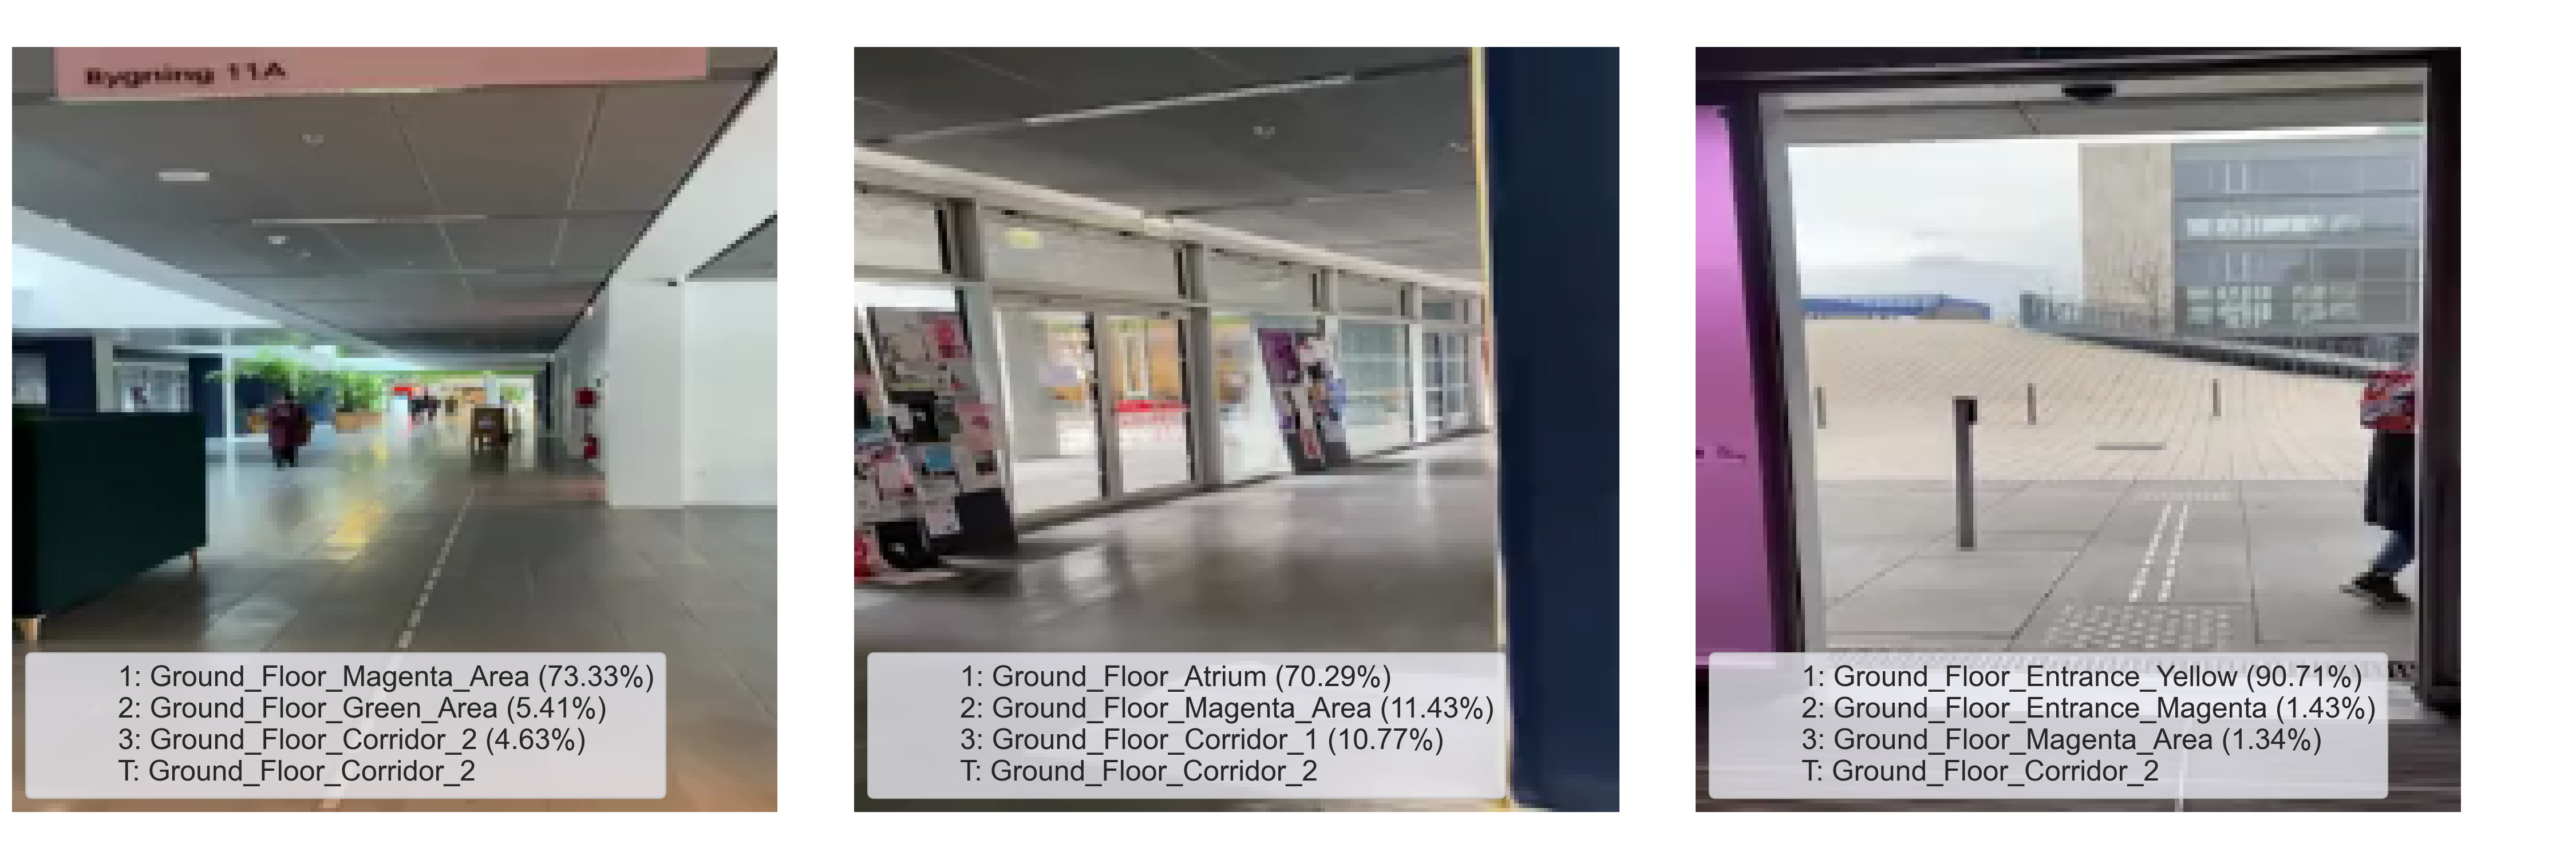
\includegraphics[width=\textwidth]{./figures/r2plus1d-mispredicted-frames.png}
      \caption{R(2+1)D}
    \end{subfigure}
    \caption{\textbf{Mispredicted Samples.} The Figure shows the mispredicted
      samples for (a) ResNet18 and (b) R(2+1)D. The respective legend shows the
      top 3 predicted classes for each sample in order of confidence and the
      ground truth label. For the clips from the video classifier, the first
      frame of the clip is shown.}
    \label{fig:mispredicted}
  \end{figure}
  
  % subsection mispredicted (end)

  \subsection{Understanding Model Behaviour: Manual Inspection} % (fold)
  \label{sub:manual}

  Finally, the continuous predictions of the two best performing model, ResNet18
  and R(2+1)D, are manually inspected on all videos in the test split. The
  following qualitative observations were made:

  \begin{enumerate} 

    \item \textbf{Prediction Robustness.} Both models show a high robustness to
      temporal changes in the environment, such as changing lighting conditions,
      different people in the scene or occlusions. This is especially true for
      R(2+1)D, which is likely due to the temporal modelling capabilities of the
      model. However, drastic changes in the environment, such as the repainting
      of an entire region, lead to consistent mispredictions of the affected
      area. This is a general drawback of localisation systems that solely rely
      on the modality of vision. A noticeable difference in terms of the
      sample-to-sample variance could be observed. ResNet18 is more prone
      "jittering" predictions. This means that for challenging subclips, the
      model is unsure about the prediction and the frame-by-frame prediction
      changes a lot. Similar behaviour was almost entirely absent in R(2+1)D.

    \item \textbf{Low-Resource Classes.} Both models struggle with classes that
      were underrepresented in the training data. This is also true for unusual
      routes and angles in the areas - the models struggle the more the testing
      clips deviate from the training data. It is hypothesised that performance
      generally improves with more versatile training data. In contrast, classes
      that show distinctive features, such as the Atrium or First Floor
      Mezzanine, are predicted more reliably.

    \item \textbf{Training Data Bias.} A bias toward the training data is
      present in both models. If features that are not representative of a
      class, but are overrepresented in the training data of that class, there
      is a chance for the model to learn these features as being indicative of a
      class. This was the case for the libraries: Most video clips that were
      taken while walking through bookshelves were filmed in library 2, while
      the other libraries were filmed in a more open space. This led to model
      associating in-between bookshelves clips to library 2, even though they
      are also present in the other libraries.

  \end{enumerate}

  % subsection manual (end)

  \subsection{Deployment on Mobile Devices}
  \label{sub:deploment}

  \begin{minipage}{0.6\textwidth}
    As a proof of concept, the best-performing model, was deployed on a mobile
    device. The trained model was first quantised to 8-bit float precision and
    then converted to \texttt{TorchScript} format. The \texttt{TorchScript} model
    was then deployed on a mobile device using the \texttt{PlayTorch}
    framework~\textit{[CITE]}. The \texttt{PlayTorch} framework is a port of the
    PyTorch Mobile SDK that is natively compatible with native iOS and Android
    Deployment to Javascript. This allows for rapid prototyping and deployment of
    PyTorch models on mobile device using the popular React Native framework and
    Expo. The model runs locally on the device and therefore does not require any
    internet connection after initially downloading the model upon opening the
    app.
  \end{minipage}
  \hfill%
  \begin{minipage}{0.3\textwidth}
    
\includegraphics[width=\linewidth]{./figures/playtorch-qr.png}
  \end{minipage}%

  % subsection deployment (end)

  % section Results (end)

  \section{Limitations \& Future Work} % (fold)
  \label{sec:discussion}

  This study has shown the potential of using a pure deep learning pipeline for
  tackling the problem of indoor localisation. However, there are still many
  open questions that need to be addressed in future work for systems similar to
  the approach suggested here to be widely useful in real-world applications.

  % coarse location labels
  The main drawback of the proposed approach is the coarse location labels.
  State-of-the-art indoor localisation systems are able to localise users to
  centimetre accuracy. Therefore, future work should focus making improvements
  on the entire pipeline that allow for higher precision in the location labels.

  % small data set
  Furthermore, this study assumes a small data set of only 40 minutes of video
  footage for training. While the experiment setup allowed to draw conclusion
  about the data efficiency of the models and the general feasibility of the
  data collection and annotation process, it is an open question how similar
  systems scale to even larger indoor spaces with more training data available.

  % representativeness of test split
  Additionally, it has to be noted that the test split was collected over a
  duration of four different days in close succession. Therefore, the test split
  might not be representative of the true variation of visual inputs from a
  indoor location over the course of a year. For example, the location might
  change more significantly than represented in the test split over seasons.
  In that case, the reported test metrics are likely to be over-optimistic. To
  gain confidence in favour or against this hypothesis, monitoring the
  performance of the trained models on test data collected over a longer period
  of time would be necessary.

  % edge-cases
  Finally, the detailed analysis of the mispredicted samples has shown that
  most errors, because the models that show a lot of similar features, such as
  different libraries, or rooms that are architecturally similar across floors.
  Future work should specifically improve on finding solutions to these issues.
  Possible starting points might be to use the fact that sudden jumps in the
  building are impossible, so highly confident predictions from the past can be
  used as a strong indicator for the next room if some knowledge about the
  relative position of the rooms is available.

  % section Discussion (end)

  \section{Conclusion} % (fold)
  \label{sec:conclusion}

  We have shown that the problem of indoor localisation can be phrased as a
  classification problem and be solved through the use of deep learning models
  in a data-efficient manner.
  Simple convolutional neural architectures were able to provide accurate and
  robust predictions and showed emerging learning of features mostly invariant
  to natural variations in the environment.
  The use of a recurrent neural network architecture allowed for the
  incorporation of temporal information and improved the accuracy of the
  predictions, though only marginally so.

  % section conclusion (end)

  % bibliography
  \newpage
  \bibliography{references}
  \bibliographystyle{abbrv}


  \newpage
  \section{Appendix} % (fold)
  \label{sec:appendix}

  \subsection{Reproducibility} % (fold)
  \label{sub:reproducibility}

  All code and data used in this project is available on GitHub at the
  following link: \url{https://github.com/mikasenghaas/bsc}. The project's 
  \texttt{README} file contains detailed instructions on how to reproduce the
  results of this project.

  Further, the precise configuration and results of the experiments that are
  reported here are publicly available on the Weights \& Biases platform at the
  following link:\\
  \url{https://wandb.ai/mikasenghaas/bsc}.

  % subsection reproducibility (end)

  \subsection{Machine Specifications} % (fold)
  \label{sub:machine-specs}

  Table~\ref{tab:machine-specs} lists the specifications of the machine that was
  used for training and evaluation of the models. For training the \texttt{MPS}
  backend was used for accelerated training. However, for inference a single CPU
  core was used, to approximate latency and throughput on mobile devices.


  \begin{table}[ht]
    \centering
    \begin{tabular}{cll}
     \toprule
     & Specification & Value \\
     \midrule

     \multirow{2}{*}{System} & Name & Darwin \\
     \vspace{0.1cm}
     & Node & Local MacBook Pro \\

     \multirow{4}{*}{CPU} & Model & Apple M1 \\
     & Architecture & ARM64 \\
     & Physical Cores & 8 \\
     \vspace{0.1cm}
     & Frequency & 2.4 GHz \\

     \multirow{2}{*}{Memory} & Total Capacity & 16 GB \\
     & Avg. Used Capacity & $\sim 7.4$ GB \\

     \bottomrule
    \end{tabular}
    \caption{Machine Specifications}
    \label{tab:machine-specs}
  \end{table}
  
  % subsection subsection name (end)

  % section remarks (end)

  \newpage
  \restoregeometry

  % encoding 
  \begin{table}[ht]
    \centering
    \begin{tabular}{lc}
    \toprule
    \bfseries Class & \bfseries Encoding \\
    \midrule
    First\_Floor\_Corridor\_1 & A \\
    First\_Floor\_Corridor\_2 & B \\
    First\_Floor\_Green\_Area & C \\
    First\_Floor\_Library\_1 & D \\
    First\_Floor\_Library\_2 & E \\
    First\_Floor\_Library\_3 & F \\
    First\_Floor\_Magenta\_Area & G \\
    First\_Floor\_Mezzanine & H \\
    First\_Floor\_Red\_Area & I \\
    First\_Floor\_Yellow\_Area & J \\
    Ground\_Floor\_Atrium & K \\
    Ground\_Floor\_Corridor\_1 & L \\
    Ground\_Floor\_Corridor\_2 & M \\
    Ground\_Floor\_Entrance\_Magenta & N \\
    Ground\_Floor\_Entrance\_Yellow & O \\
    Ground\_Floor\_Green\_Area & P \\
    Ground\_Floor\_Magenta\_Area & Q \\
    Ground\_Floor\_Red\_Area & R \\
    Ground\_Floor\_Yellow\_Area & S \\
    Stairs\_Atrium & T \\
    \bottomrule
    \end{tabular}
    \caption{Encoding of Classes}
    \label{tab:class-encoding}
  \end{table}

  % section appendix (end)
  

\end{document}
